\documentclass[conference]{IEEEtran}
\IEEEoverridecommandlockouts

\usepackage{fontspec}
\setmainfont{Times New Roman}
\setsansfont{Times New Roman}
\setmonofont{Times New Roman}

\usepackage{graphicx}
\usepackage{booktabs}
\usepackage{array}
\usepackage{amsmath,amssymb}
\PassOptionsToPackage{hyphens}{url}
\usepackage[hidelinks]{hyperref}
\urlstyle{same}
\def\UrlBreaks{\do\/\do-\do_\do.}

\AtBeginDocument{%
  \renewcommand{\figurename}{Hình}
  \renewcommand{\tablename}{BẢNG}
  \renewcommand{\refname}{TÀI LIỆU THAM KHẢO}
  \renewcommand{\abstractname}{Tóm tắt}
  \renewcommand{\IEEEkeywordsname}{Từ khóa}
}

\setlength{\emergencystretch}{2.5em}
\sloppy
\setlength{\textfloatsep}{7pt plus 2pt minus 2pt}
\setlength{\dbltextfloatsep}{7pt plus 2pt minus 2pt}
\setlength{\intextsep}{6pt plus 2pt minus 2pt}
\setlength{\abovecaptionskip}{3pt}
\setlength{\belowcaptionskip}{1pt}

\IEEEpubid{\makebox[\columnwidth]{FIT4013 -- Nhập môn Học máy | Khoa CNTT, Trường Đại học Đại Nam \copyright 2026 Nhóm 6\hfill}\hspace{\columnsep}\makebox[\columnwidth]{}}

\begin{document}

\title{Nhận Dạng Biển Báo Giao Thông Trên Bộ Dữ Liệu GTSRB: Đánh Giá Thực Nghiệm Đặc Trưng HOG, Màu Sắc, Giảm Chiều PCA Và Các Thuật Toán Học Máy}

\author{%
\IEEEauthorblockN{Lê Trọng Chiến\textsuperscript{*} (Trưởng nhóm), Đặng Việt Anh\textsuperscript{\textdagger}, Nguyễn Hữu Dũng\textsuperscript{\textdaggerdbl}, Kiều Văn Nam\textsuperscript{\S}}
\IEEEauthorblockA{Khoa Công nghệ Thông tin, Trường Đại học Đại Nam, Hà Nội, Việt Nam (Lớp CNTT 18-10 -- Nhóm 6)\\
MSV: \textsuperscript{*}1871020089 (Trưởng nhóm), \textsuperscript{\textdagger}1871020683, \textsuperscript{\textdaggerdbl}1871020172, \textsuperscript{\S}1871020416 --- GVHD: ThS. Lê Thị Thùy Trang\\
Email: 1871020089@dnu.edu.vn, 1871020683@dnu.edu.vn, 1871020172@dnu.edu.vn, 1871020416@dnu.edu.vn}
}

\maketitle

\begin{abstract}
Báo cáo này xây dựng và đánh giá quy trình học máy hoàn chỉnh để phân loại 43 loại biển báo giao thông trên toàn bộ 51.839 ảnh của bộ dữ liệu GTSRB, thực thi tái lập trên môi trường CPU của Google Colab. Nhằm loại bỏ hoàn toàn hiện tượng rò rỉ dữ liệu theo chuỗi khung hình liên tiếp (track) giữa tập huấn luyện và tập kiểm định, nhóm áp dụng phân tách StratifiedGroupKFold theo mã track vật lý (1.045 track huấn luyện so với 262 track kiểm định, không có track trùng lặp) và chỉ dùng tập kiểm định nhóm (GroupVal) để chọn siêu tham số trước khi đánh giá một lần cuối trên 12.630 ảnh Test độc lập. Kết quả cho thấy bước trích xuất đặc trưng HOG sau cắt vùng quan tâm ROI và cân bằng sáng cục bộ CLAHE là nhân tố quyết định nâng K-NN từ 50,59\% (Baseline pixel xám F1) lên 89,86\% (HOG F3) và 90,45\% sau nén PCA 128 chiều (F3-PCA, k=11). Ngược lại, việc ghép thêm 96 chiều màu vào K-NN làm giảm nhẹ độ chính xác xuống 89,79\% (kiểm định McNemar p = 0,0004) do chuẩn hóa phương sai đồng mức giữa các kênh màu với gradient cạnh, trong khi hỗ trợ tích cực cho Cây quyết định (tăng từ 72,05\% lên 72,32\%) và Gaussian Naive Bayes trên không gian PCA (88,20\%, suy luận 0,35 giây). Mô hình mở rộng MLP trên F5 đạt đỉnh 92,77\% ($\pm$ 0,46\%, Macro-F1 89,96\%). Hệ thống còn tích hợp phân tích lỗi định lượng theo kích thước, độ sáng, đường cong Coverage--Accuracy và thiết kế ứng dụng Web Demo đa mô hình theo kiến trúc mô-đun bằng Python Flask.
\end{abstract}

\begin{IEEEkeywords}
Nhận dạng biển báo giao thông, GTSRB, StratifiedGroupKFold, HOG, CLAHE, PCA, K-NN, Decision Tree, Gaussian Naive Bayes, MLP.
\end{IEEEkeywords}

% ==================== SECTION I ====================
\section{ĐẶT VẤN ĐỀ VÀ PHÂN TÍCH YÊU CẦU}

\subsection{Bối cảnh và mục tiêu nghiên cứu}
Trong các hệ thống hỗ trợ lái xe nâng cao (ADAS) và xe tự hành, nhận dạng chính xác biển báo giao thông từ camera hành trình giữ vai trò cốt lõi để cảnh báo giới hạn tốc độ, chỉ dẫn bắt buộc hoặc nguy hiểm phía trước~\cite{stallkamp2012man}. Ảnh thu ngoài trời thường chịu biến thiên mạnh về khoảng cách chụp (khiến chữ số rất nhỏ), điều kiện thiếu sáng hoặc chói sáng, nhòe chuyển động và hậu cảnh phức tạp.

Báo cáo thực hiện quy trình học máy cổ điển có khả năng tái lập cao trên bộ dữ liệu chuẩn GTSRB (43 lớp) với bốn đóng góp trọng tâm:
\begin{enumerate}
  \item Phát hiện và xử lý triệt để rò rỉ dữ liệu theo chuỗi khung hình (track leakage) khi phân tách tập huấn luyện/kiểm định bằng phương pháp StratifiedGroupKFold~\cite{kaufman2012leakage,pedregosa2011scikit}, đồng thời khóa kín tập Test độc lập trong suốt quá trình tinh chỉnh tham số.
  \item Thực hiện đánh giá tách bạch (ablation study) 8 tầng đặc trưng từ pixel thô đến HOG, đặc trưng màu sắc HSV/RGB, CLAHE và giảm chiều PCA trên cả ba thuật toán cốt lõi của học phần là K-NN, Cây quyết định (Decision Tree) và Gaussian Naive Bayes.
  \item Đánh giá độ tin cậy thực nghiệm bằng khoảng tin cậy Bootstrap 95\% (1.000 lần lấy mẫu lại) và kiểm định thống kê McNemar, khắc phục tình trạng diễn giải các chênh lệch ngẫu nhiên dưới mức sai số chuẩn.
  \item Thực hiện đối sánh mở rộng với Random Forest và mạng nơ-ron đa tầng (MLP), kiểm chứng định lượng nguyên nhân lỗi theo kích thước, độ sáng, đường cong Coverage--Accuracy và thiết kế ứng dụng Web Demo mô-đun bằng Python Flask.
\end{enumerate}

\subsection{Nguồn dữ liệu, bản quyền và phân tích khám phá (EDA)}
\IEEEpubidadjcol
Bộ dữ liệu GTSRB (German Traffic Sign Recognition Benchmark)~\cite{stallkamp2011german,stallkamp2012man} được công bố công khai phục vụ mục đích nghiên cứu học thuật (tại kho dữ liệu gốc của Viện Thần kinh Tin học Ruhr-Universität Bochum qua cổng lưu trữ \url{https://sid.erda.dk/public/archives/daaeac0d7ce1152aea9b61d9f1e19370/} và bản phản chiếu Kaggle \url{https://www.kaggle.com/datasets/meowmeowmeowmeowmeow/gtsrb-german-traffic-sign}, áp dụng giấy phép dữ liệu công cộng/nghiên cứu CC0). Dữ liệu gồm tổng cộng 51.839 ảnh RGB thuộc 43 lớp: 39.209 ảnh tập huấn luyện gốc (Train) và 12.630 ảnh tập kiểm thử độc lập (Test). Mỗi bản ghi siêu dữ liệu chứa kích thước ảnh (Width, Height), hộp giới hạn vùng chứa biển báo (Roi.X1, Roi.Y1, Roi.X2, Roi.Y2), nhãn lớp (ClassId $\in \{0,\dots,42\}$) và đường dẫn tệp.

Đặc thù cấu trúc quan trọng của GTSRB là tập Train được ghi từ video thành các chuỗi 30 khung hình liên tiếp (track vật lý) quay cùng một biển báo ngoài thực tế (tổng cộng 1.307 track: 1.306 track đủ 30 ảnh và 1 track cuối gồm 29 ảnh), còn tập Test gồm các track thu thập riêng biệt trên tuyến đường và thời điểm khác. Kiểm tra toàn vẹn cho thấy 0 giá trị thiếu và 0 bản ghi trùng lặp.

\begin{figure*}[!t]
\centering
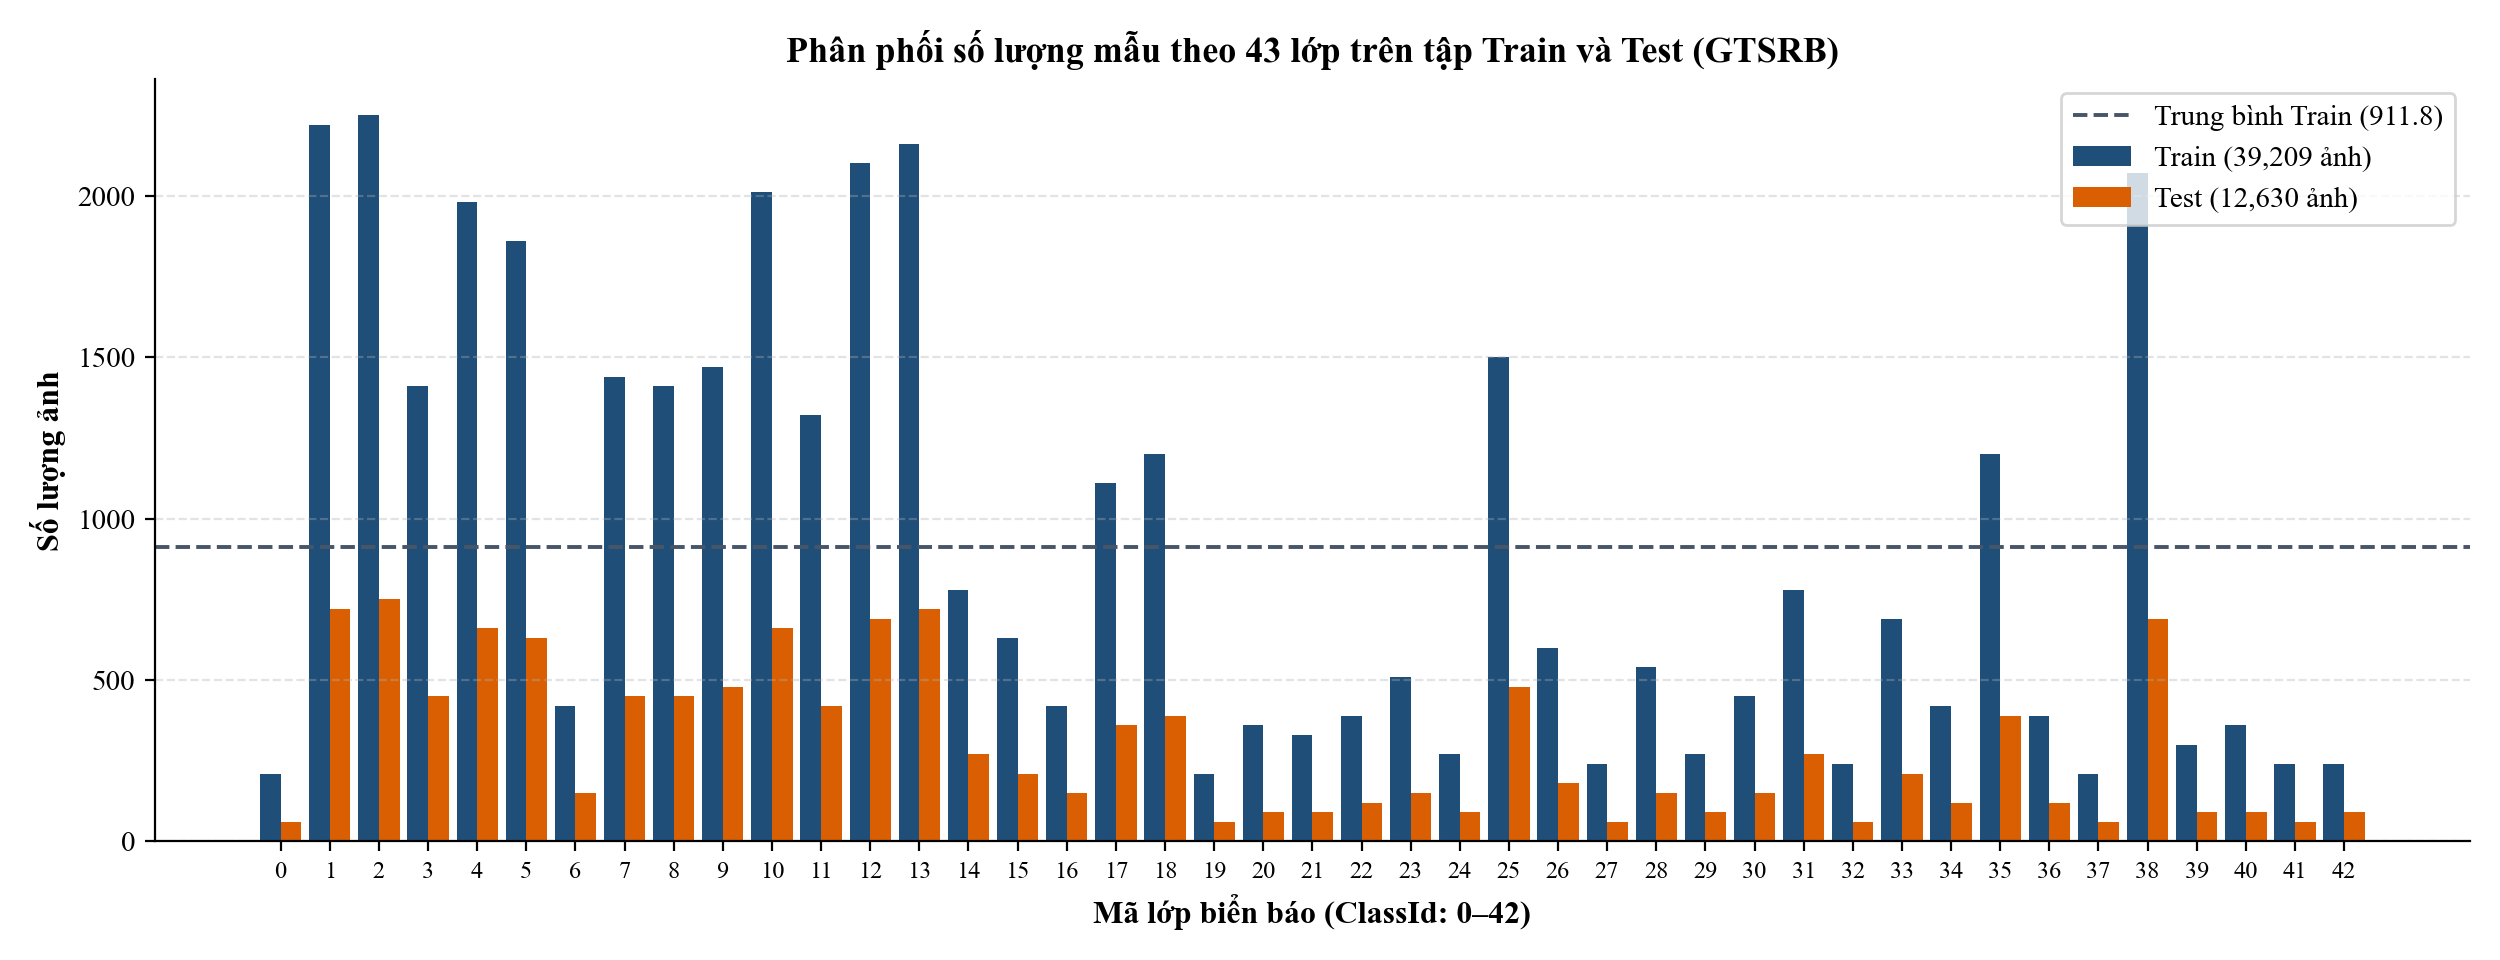
\includegraphics[width=0.45\textwidth]{figures/fig1_class_distribution.png}\hfill
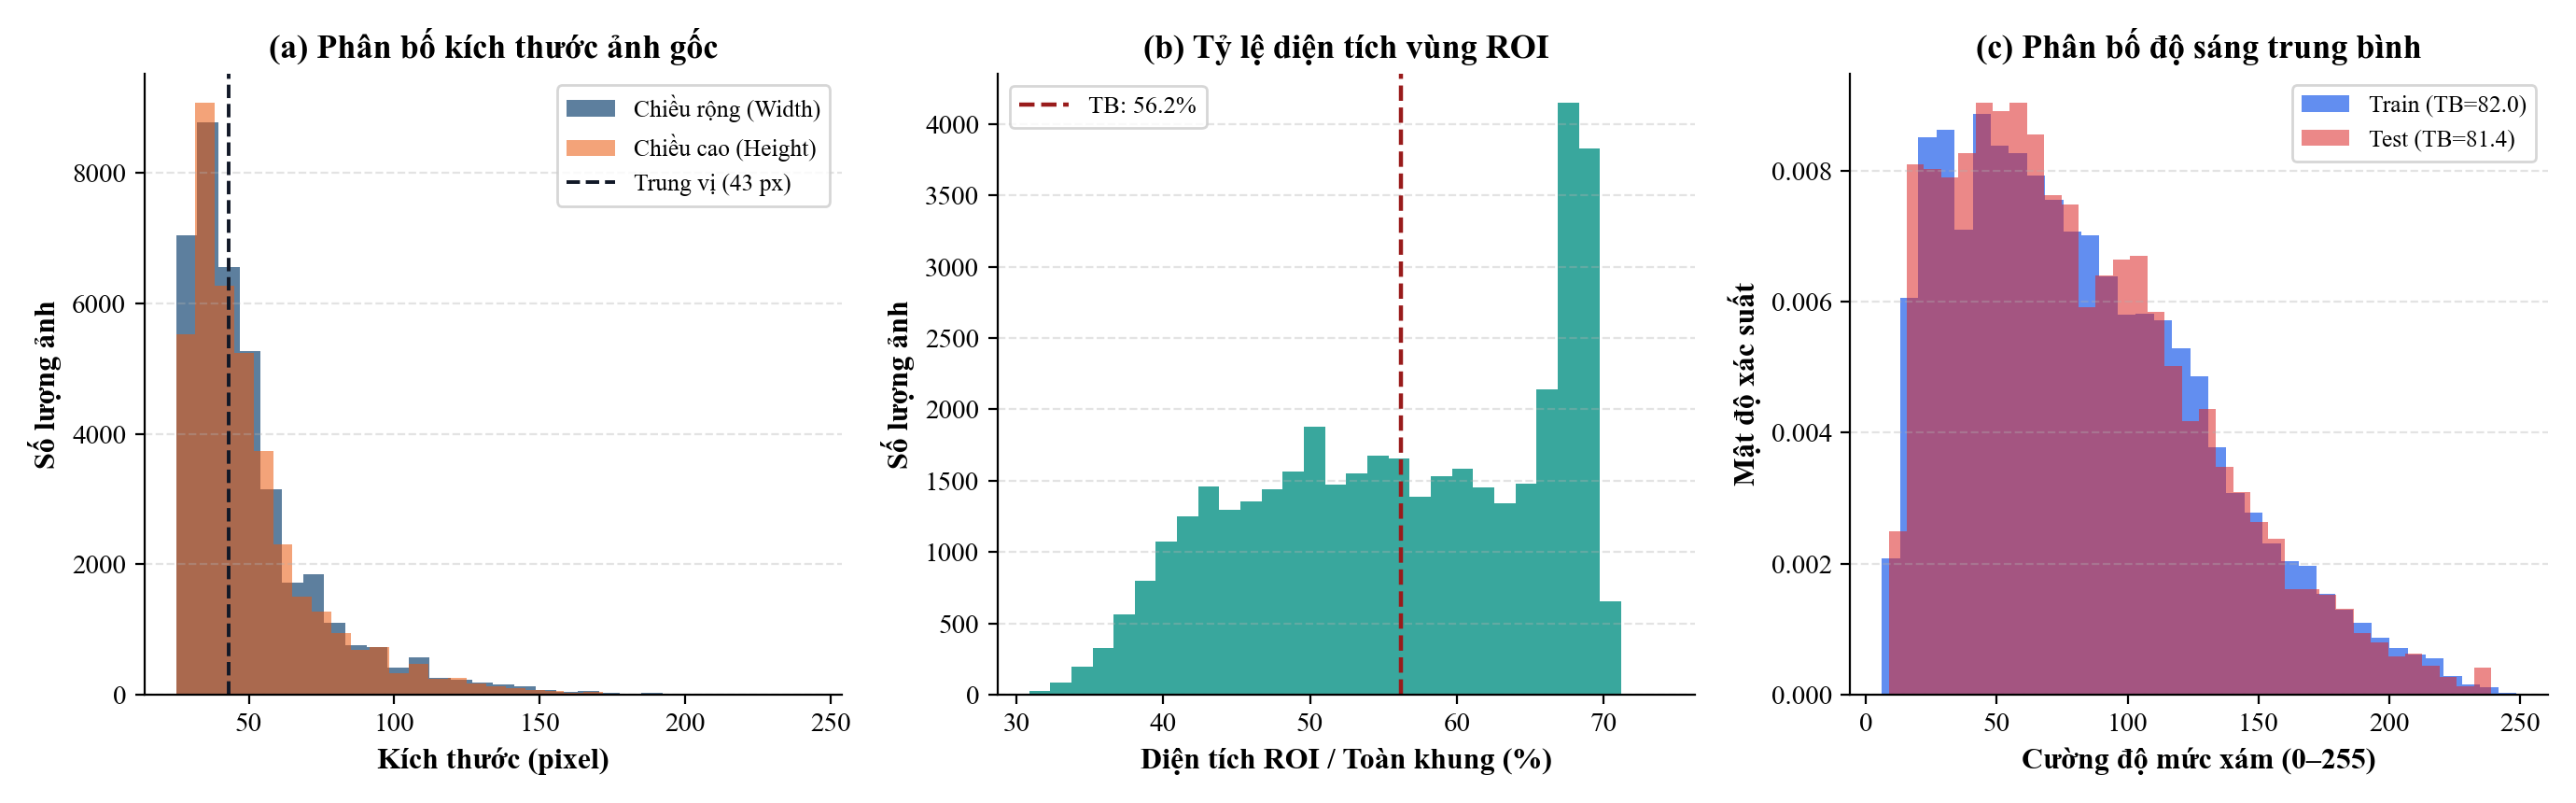
\includegraphics[width=0.53\textwidth]{figures/fig3_eda_dimensions_brightness.png}
\caption{Kết quả khám phá dữ liệu trên 51.839 ảnh GTSRB: (trái) phân phối mất cân bằng theo 43 lớp; (phải) phân bố kích thước ảnh gốc, tỷ lệ diện tích ROI và phân phối độ sáng trung bình trên tập Train và Test.}
\label{fig:eda}
\end{figure*}

\begin{figure*}[!t]
\centering
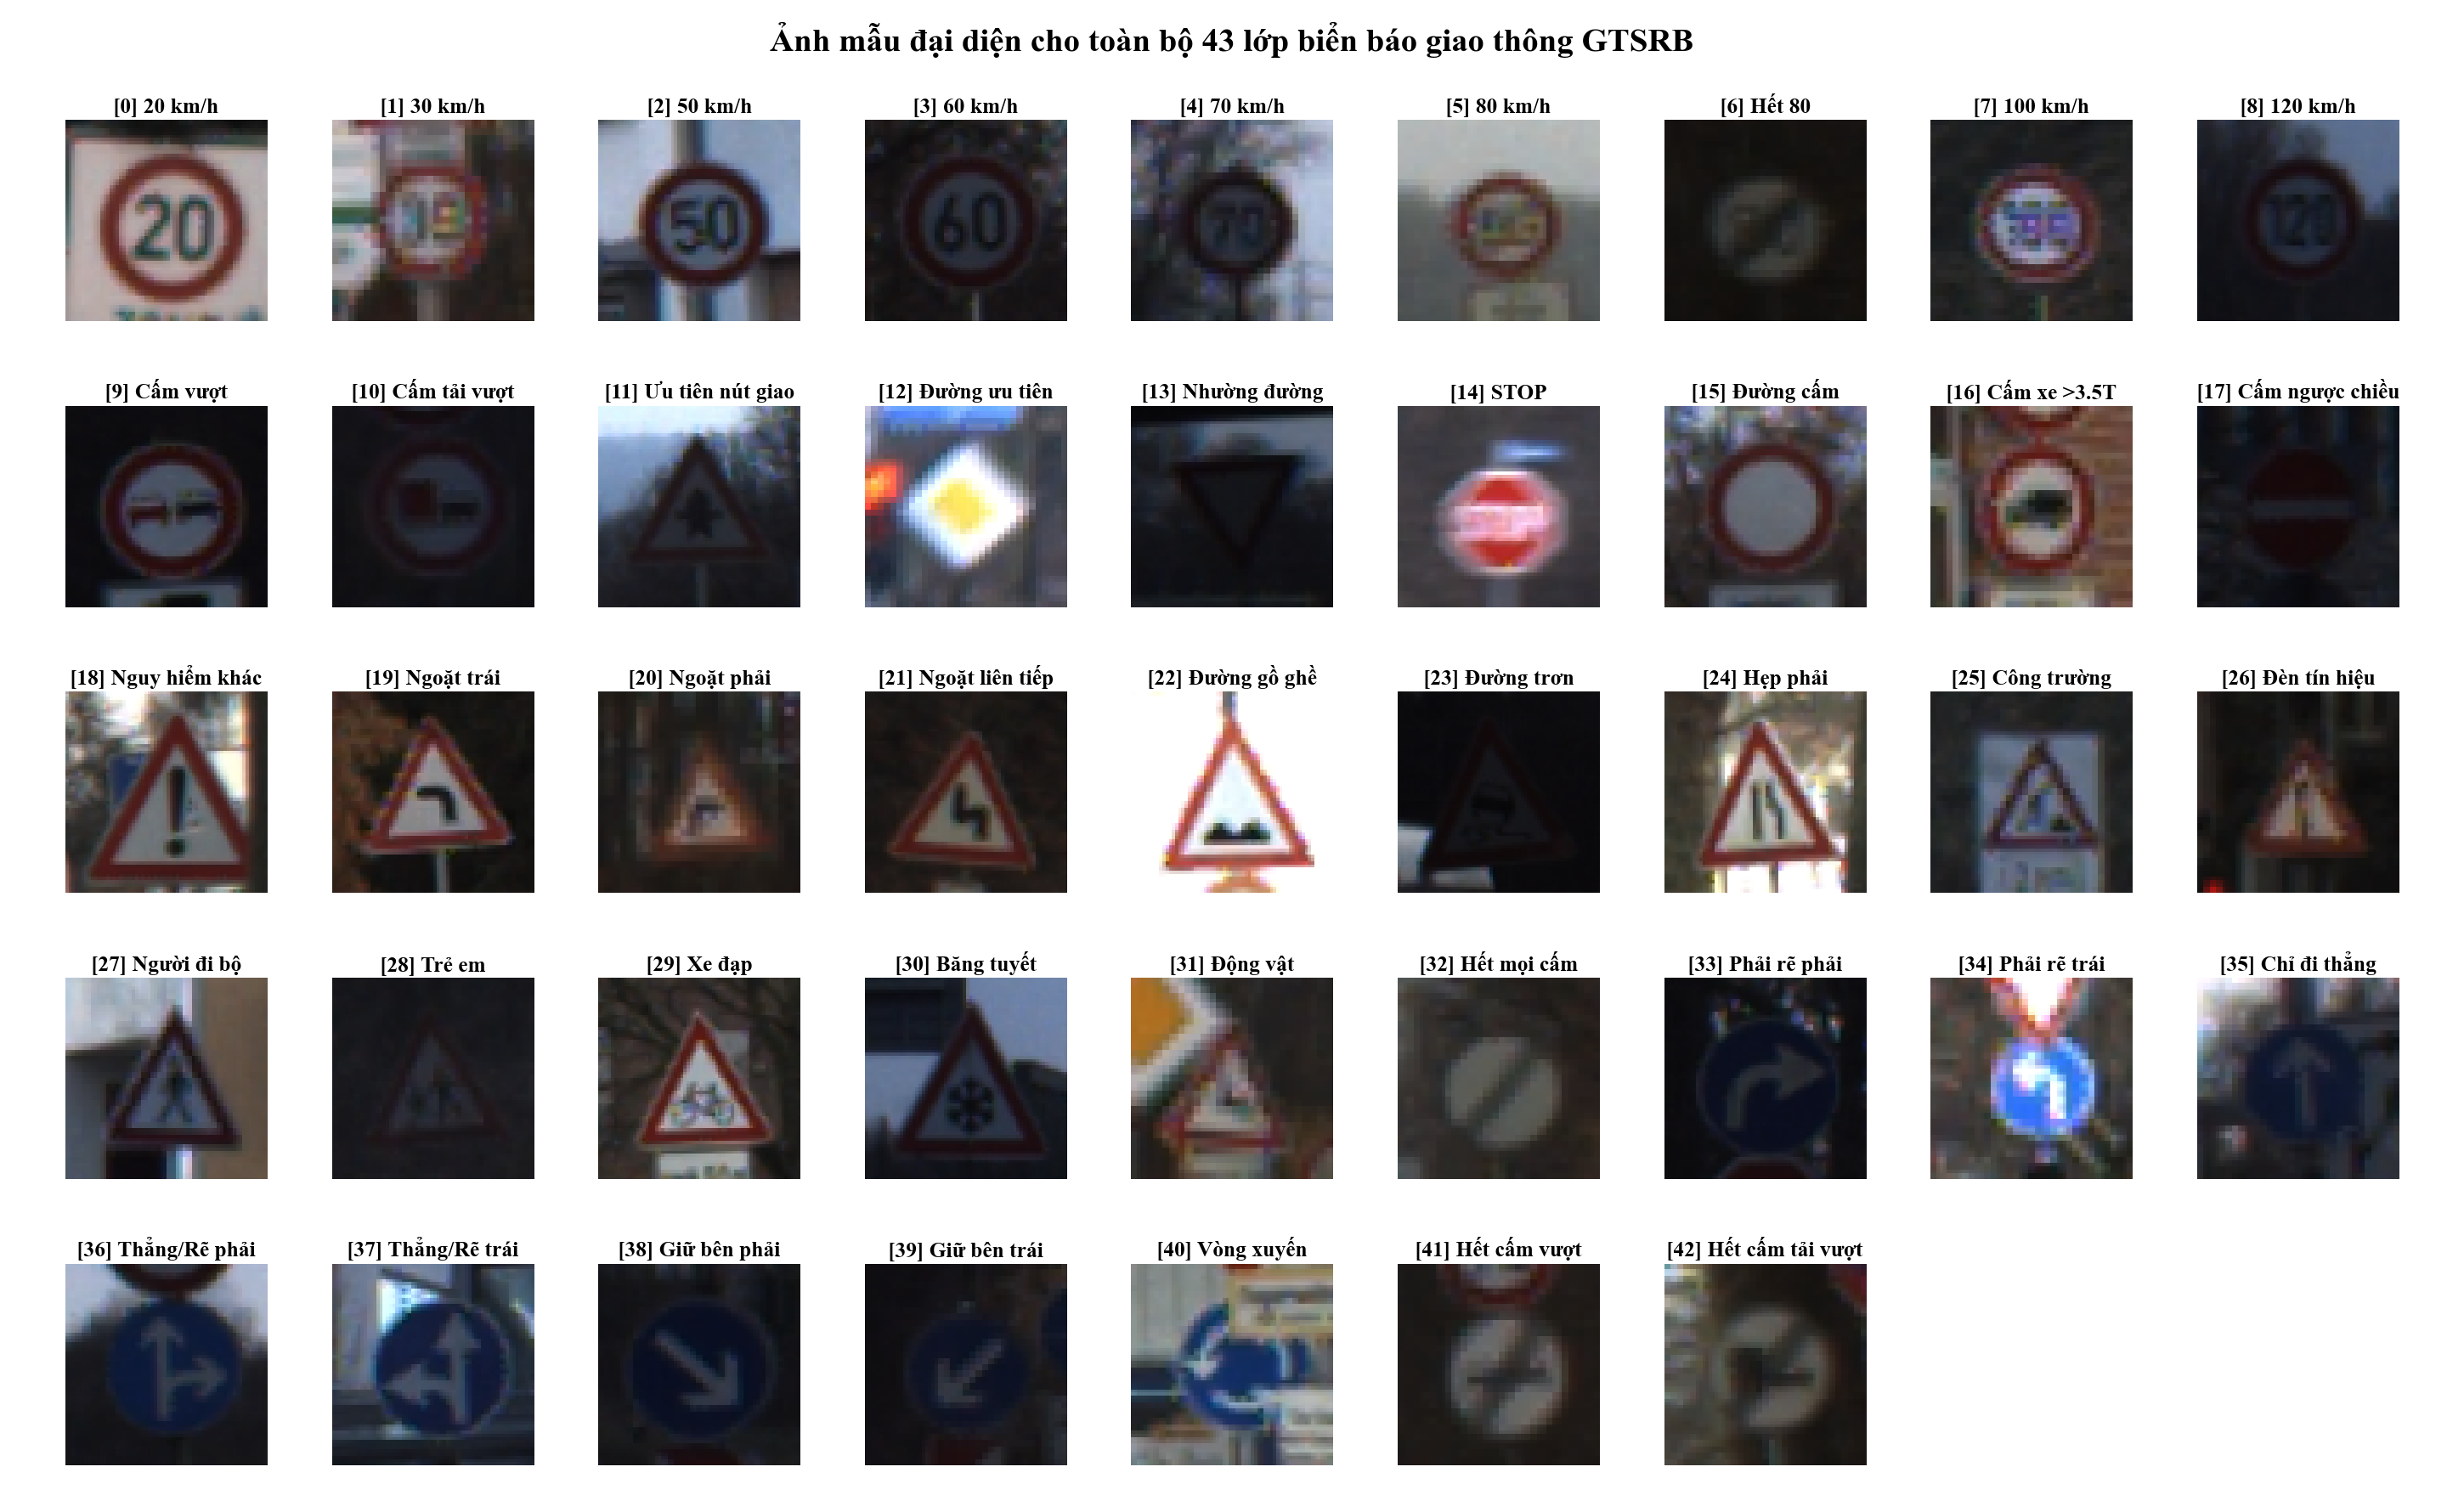
\includegraphics[width=0.86\textwidth]{figures/fig2_sample_grid_43classes.png}
\caption{Ảnh mẫu thực tế đại diện cho toàn bộ 43 lớp biển báo giao thông trong tập dữ liệu GTSRB (Lớp 0 đến Lớp 42).}
\label{fig:grid43}
\end{figure*}

Hình~\ref{fig:eda} và Hình~\ref{fig:grid43} phản ánh ba tính chất nổi bật từ bước EDA:
\begin{itemize}
  \item Mất cân bằng lớp (tỷ lệ 10,7:1): Tập Train có trung bình 911,8 ảnh/lớp; các lớp thiểu số nhất (Lớp 0, Lớp 19 và Lớp 37) chỉ có 210 ảnh, trong khi Lớp 2 đạt 2.250 ảnh (tập Test dao động từ 60 đến 750 ảnh/lớp). Do đó, báo cáo đánh giá đồng thời Accuracy và các chỉ số Macro Precision, Macro Recall, Macro F1-score~\cite{powers2020evaluation}.
  \item Nhiễu hậu cảnh ngoài ROI: Kích thước ảnh gốc dao động từ $25\times 25$ đến $243\times 225$ pixel (trung vị $43\times 43$ px); hộp giới hạn ROI trung bình chỉ chiếm 56,2\% tổng diện tích ảnh, đồng nghĩa khoảng 43,8\% khung ảnh gốc là hậu cảnh nhiễu cần cắt bỏ.
  \item Điều kiện ánh sáng thiên tối: Cường độ mức xám trung bình đạt 82,0 $\pm$ 47,6 trên tập Train và 81,4 trên tập Test (thang 0--255), nghiêng rõ rệt về dải ảnh tối dưới 80.
\end{itemize}

% ==================== SECTION II ====================
\section{THIẾT KẾ GIẢI PHÁP VÀ QUY TRÌNH HỌC MÁY}
Hình~\ref{fig:arch} minh họa sơ đồ kiến trúc tổng thể từ khâu thu thập dữ liệu, phân tách chống rò rỉ theo track, tiền xử lý, rút trích đặc trưng F0--F5, tinh chỉnh trên GroupVal, kiểm định một lần trên tập Test khóa cho đến thiết kế ứng dụng Demo tương tác ngoài thực tế.

\begin{figure*}[!t]
\centering
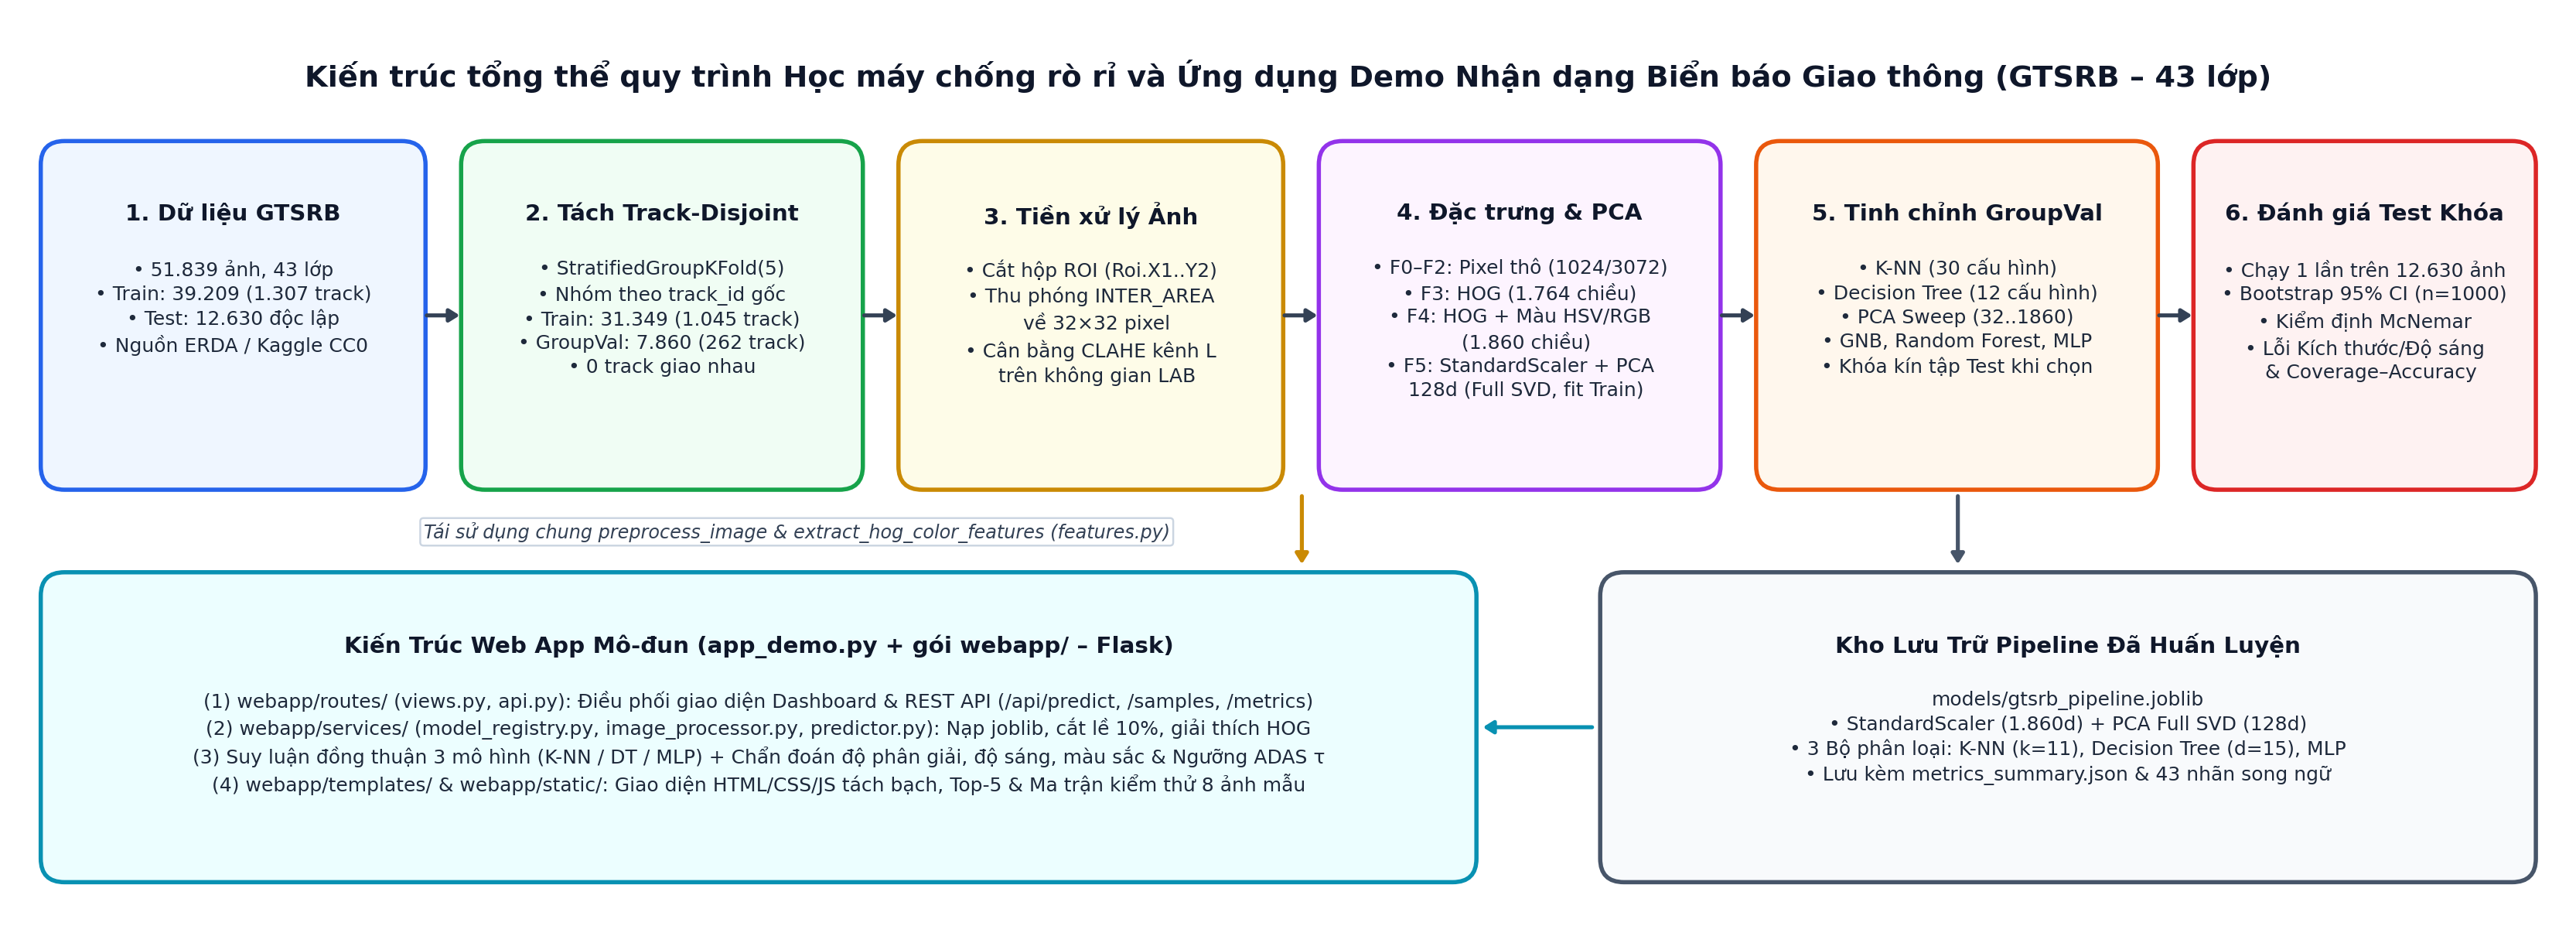
\includegraphics[width=0.90\textwidth]{figures/fig0_pipeline_architecture.png}
\caption{Kiến trúc tổng thể quy trình học máy chống rò rỉ theo track và thiết kế ứng dụng Demo nhận dạng biển báo GTSRB.}
\label{fig:arch}
\end{figure*}

\subsection{Phân tách dữ liệu theo track và chống rò rỉ dữ liệu}
Khi sử dụng hàm chia ngẫu nhiên theo từng ảnh (train\_test\_split chuẩn với seed cố định 42), các khung hình kề nhau trong cùng một track 30 ảnh bị phân tán vào cả hai tập Train và Validation. Thực nghiệm đối chứng trên cùng đặc trưng F5 (với K-NN k=5, Euclidean) chứng minh hiện tượng thổi phồng này: cách chia ngẫu nhiên theo khung hình tạo ra điểm Validation đạt 98,66\% dù Test thực tế chỉ đạt 89,75\% (chênh lệch ảo +8,91 điểm \%). Ngược lại, khi nhóm sử dụng StratifiedGroupKFold (5 phần, lấy tập kiểm định đầu tiên) nhóm theo mã track\_id, 31.349 ảnh huấn luyện thuộc 1.045 track và 7.860 ảnh kiểm định (GroupVal) thuộc 262 track hoàn toàn tách biệt (số track giao nhau bằng 0). Khi đó, điểm GroupVal đạt 91,42\%, phản ánh chân thực năng lực tổng quát hóa gần với tập Test (89,18\%).

Toàn bộ các bước học tham số thống kê gồm StandardScaler và phép chiếu PCA đều chỉ được khớp (fit) trên tập Train tách track (31.349 ảnh), sau đó biến đổi (transform) sang GroupVal và Test~\cite{kaufman2012leakage}. Algorithm~1 trình bày quy trình thực thi chuẩn, đảm bảo tập Test chỉ được đánh giá duy nhất sau khi chốt xong siêu tham số trên GroupVal.

\begin{table}[!t]
\centering
\small
\begin{tabular}{@{}p{0.96\columnwidth}@{}}
\hline
\textbf{Algorithm 1} Quy trình phân tách track không rò rỉ \\
\hline
\textbf{Input:} Tập Train (39.209 ảnh, 1.307 track), tập Test (12.630 ảnh), PCA d=128. \\
\textbf{Output:} Mô hình tối ưu, khoảng tin cậy 95\% CI và độ đo trên Test khóa. \\
1: Gán mã track\_id = ClassId + TrackPrefix cho toàn bộ 39.209 ảnh Train. \\
2: Tách StratifiedGroupKFold(5) theo track\_id $\rightarrow$ Train (31.349) và GroupVal (7.860). \\
3: Trích xuất đặc trưng F0--F4 (ROI, Resize $32\times 32$, CLAHE, HOG, HSV/RGB). \\
4: Khớp StandardScaler và PCA (svd\_solver=full) duy nhất trên dữ liệu Train. \\
5: Biến đổi dữ liệu Train, GroupVal và Test sang biểu diễn float32. \\
6: Quét lưới siêu tham số (Exp 2--4) chỉ dùng GroupVal Accuracy/Macro-F1 để chọn cấu hình. \\
7: Đánh giá một lần trên tập Test khóa (12.630 ảnh) kèm Bootstrap 95\% CI và McNemar. \\
\hline
\end{tabular}
\end{table}

\subsection{Tiền xử lý và trích xuất các tầng đặc trưng (F0--F5)}
Mỗi ảnh RGB đi qua các bước tiền xử lý chuẩn hóa tuần tự: (1) cắt theo khung ROI khi kích hoạt; (2) thu phóng đồng nhất về $32\times 32$ bằng nội suy vùng INTER\_AREA~\cite{bradski2000opencv}; (3) chuyển sang không gian màu LAB và cân bằng sáng cục bộ CLAHE (clipLimit=2,0, tileGridSize=(4,4)) trên kênh độ chói $L$~\cite{zuiderveld1994contrast} trước khi đưa về RGB (Hình~\ref{fig:preproc}). Một lưu ý kỹ thuật quan trọng là phép cân bằng CLAHE làm thay đổi trực tiếp phân phối giá trị sáng trên kênh $L$, từ đó biến đổi phân phối thành phần $V$ khi chuyển sang HSV; tác động này được kiểm chứng riêng giữa F4\_noCLAHE và F4.

Để đánh giá định lượng đóng góp từng thành phần, nhóm xây dựng 8 cấu hình biểu diễn đặc trưng (đều đi qua StandardScaler khớp trên tập Train):
\begin{itemize}
  \item F0 (1.024 chiều): Ảnh xám toàn khung $32\times 32$ không cắt ROI, chia 255 về $[0,1]$.
  \item F1 -- Baseline (1.024 chiều): Cắt ROI, resize $32\times 32$, chuyển xám và chia 255 về $[0,1]$.
  \item F2 (3.072 chiều): Ảnh màu RGB $32\times 32\times 3$ đã cắt ROI.
  \item F3 -- HOG (1.764 chiều): Rút trích biểu đồ định hướng gradient cục bộ~\cite{dalal2005histograms,walt2014scikit} trên ảnh xám sau CLAHE (9 hướng, ô $4\times 4$ px, khối $2\times 2$ ô, chuẩn hóa L2-Hys và biến đổi căn bậc hai):
  \begin{equation}
  M=\sqrt{G_x^2+G_y^2},\quad \theta=\operatorname{atan2}(G_y,G_x)
  \end{equation}
  \begin{equation}
  v_{\text{norm}} = \frac{v}{\sqrt{\|v\|_2^2 + \epsilon^2}} \qquad (\text{ngưỡng cắt } \le 0{,}2)
  \end{equation}
  \item F3-PCA (128 chiều): Nén vector F3 (1.764 chiều HOG thuần) bằng PCA chính xác (svd\_solver=full) xuống 128 chiều (giữ 64,63\% phương sai) nhằm tách riêng tác động của nén chiều với tác động của màu sắc.
  \item F4 -- HOG + Màu sắc (1.860 chiều) và F4 (Không CLAHE): Ghép 1.764 chiều HOG với 96 chiều màu sắc/cường độ sáng~\cite{bradski2000opencv} gồm: 32 ngăn biểu đồ biên HSV (16 Hue + 8 Saturation + 8 Value chuẩn hóa), 48 chiều lưới màu RGB $4\times 4$ và 16 chỉ số thống kê toàn cục (trung bình, độ lệch chuẩn RGB/HSV và 4 tỷ lệ điểm ảnh vùng đỏ, xanh lam, vàng, tối):
  \begin{equation}
  x_{\text{F4}} = \left[\,f_{\text{HOG}};\; h_{\text{HSV}};\; g_{4\times 4}^{\text{RGB}};\; s_{\text{stat}}\,\right] \in \mathbb{R}^{1860}
  \end{equation}
  \item F5 -- F4 + PCA (128 chiều): Chuẩn hóa vector F4 qua StandardScaler và chiếu qua 128 thành phần chính (svd\_solver=full, giữ 64,74\% tổng phương sai)~\cite{jolliffe2016principal}:
  \begin{equation}
  z = \tilde{x}W_d, \qquad \text{EVR}(d) = \frac{\sum_{i=1}^d \lambda_i}{\sum_{j=1}^D \lambda_j}
  \end{equation}
\end{itemize}

\begin{figure}[!t]
\centering
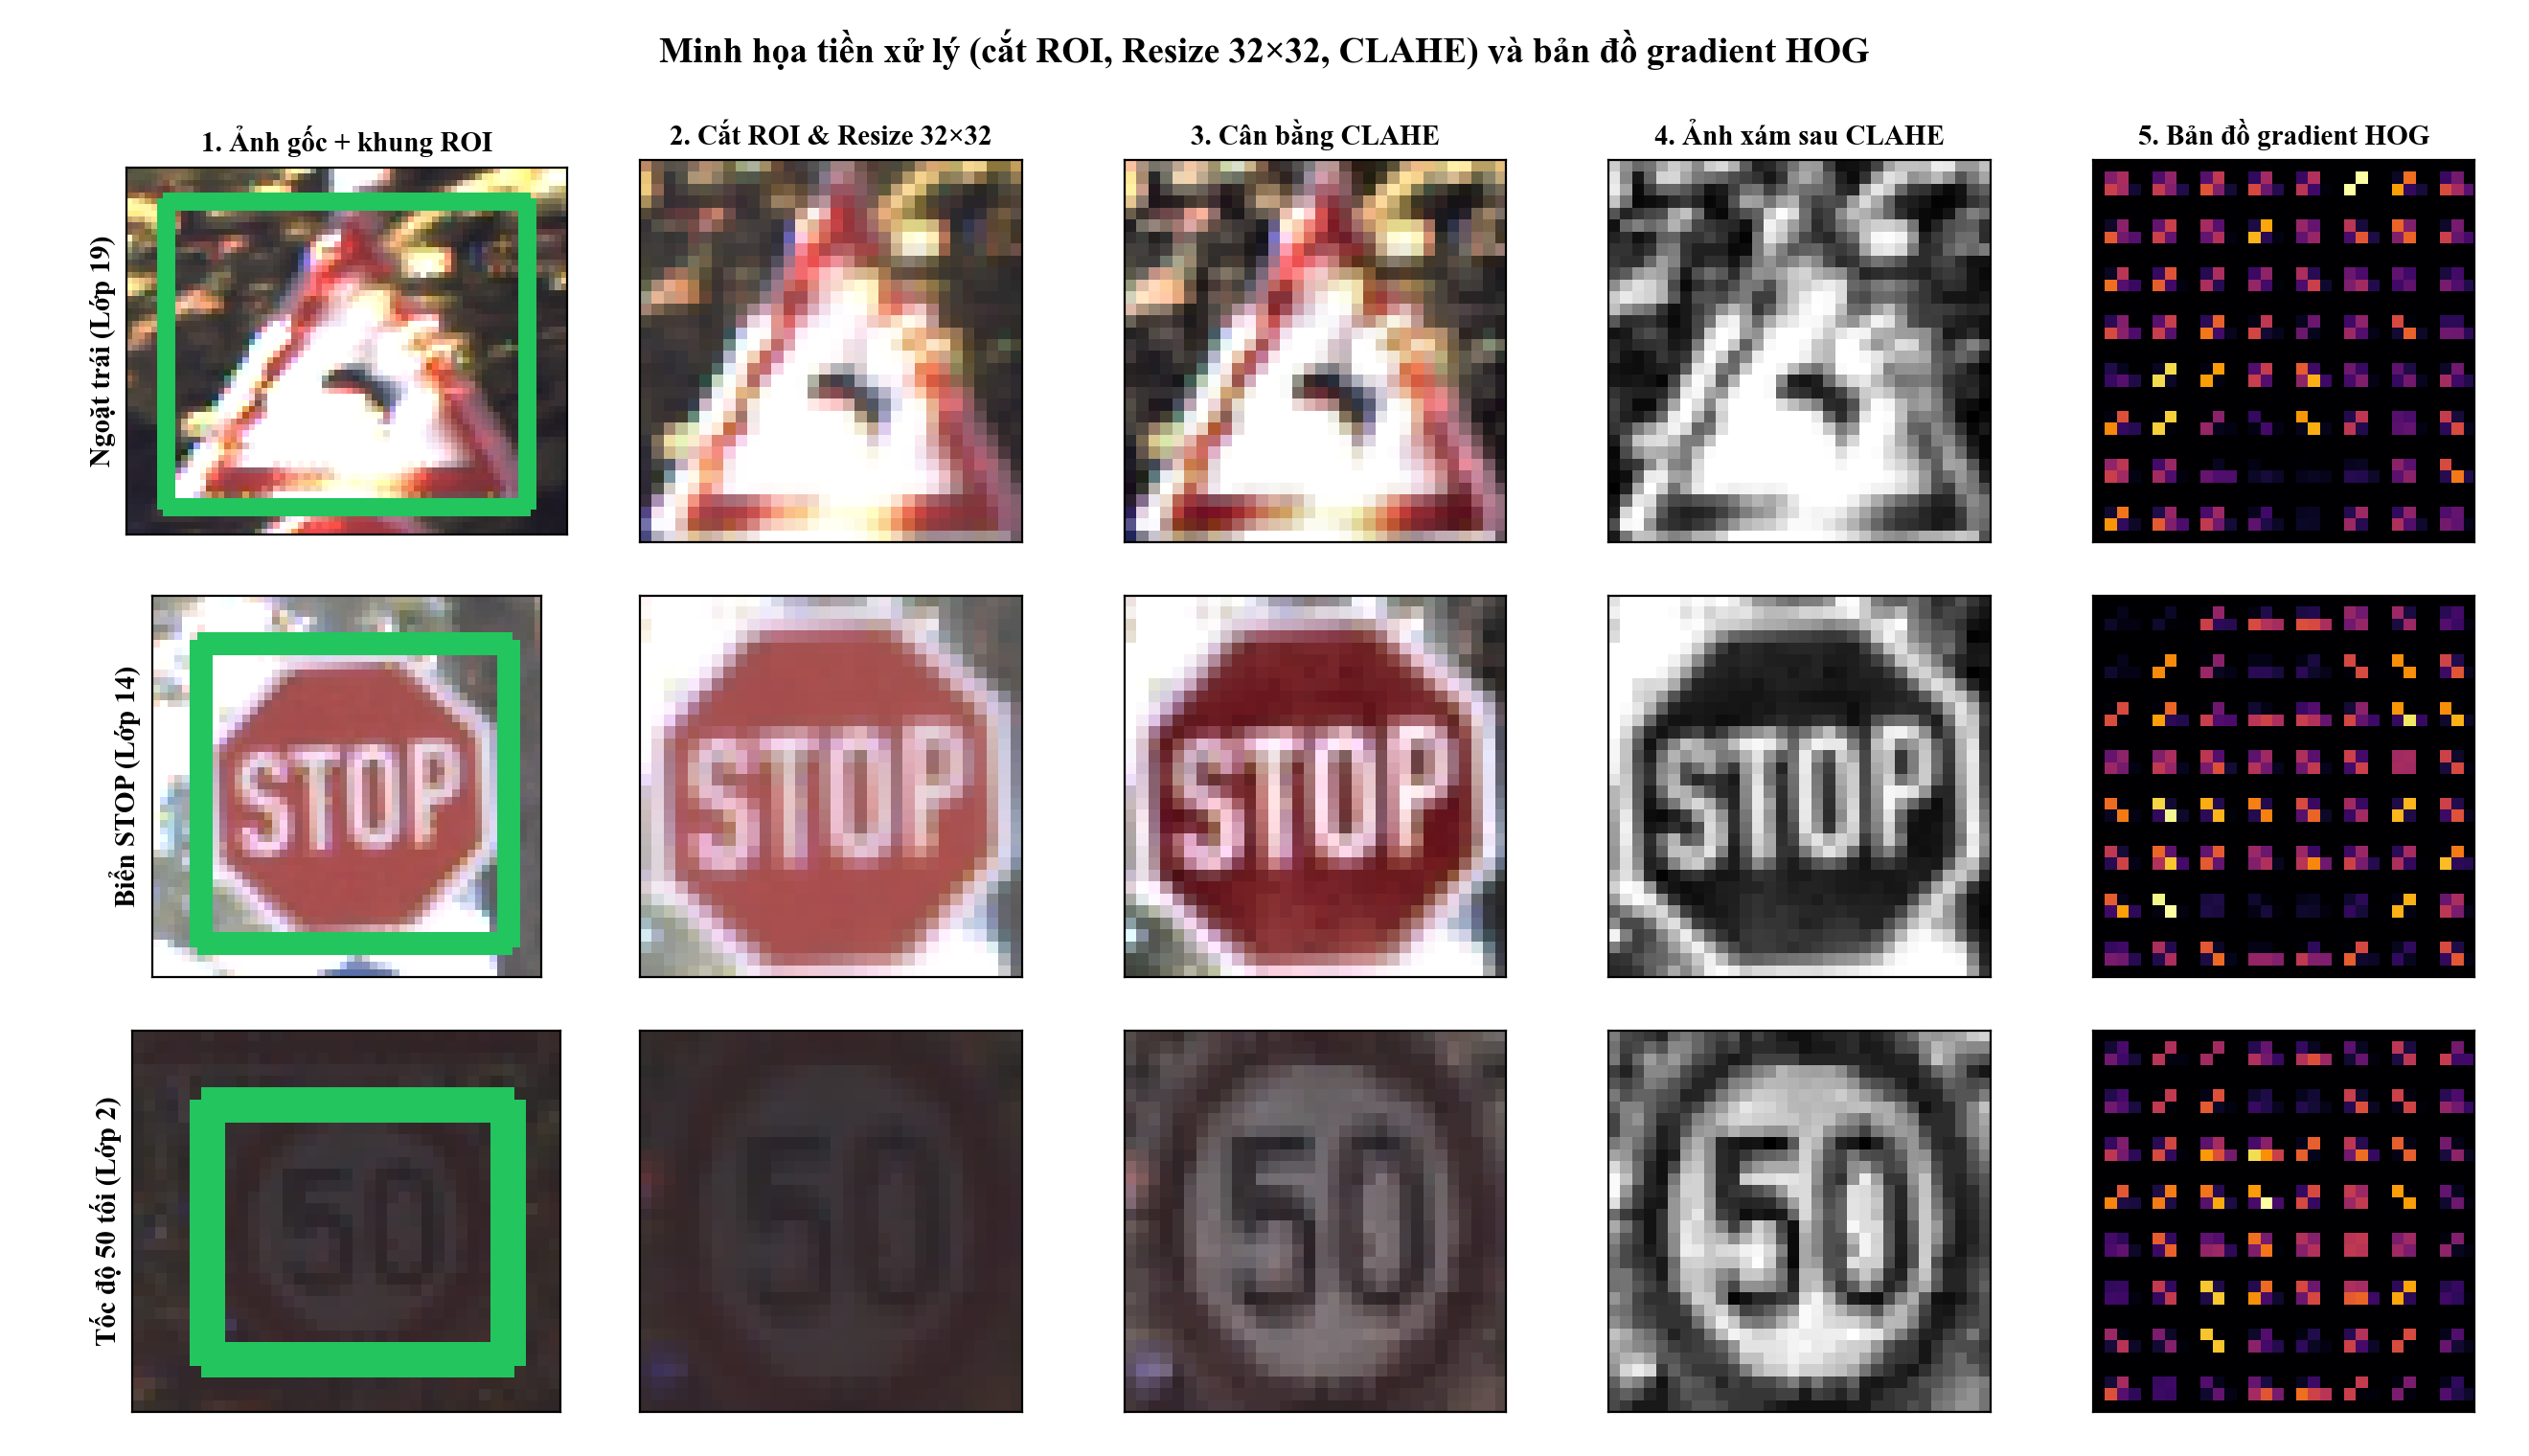
\includegraphics[width=\columnwidth]{figures/fig4_preprocessing_hog_pipeline.png}
\caption{Minh họa từng bước tiền xử lý (cắt ROI, Resize $32\times 32$, CLAHE) và bản đồ gradient HOG trên 3 mẫu biển báo GTSRB thuộc Lớp 19, Lớp 14 (STOP) và Lớp 2 (50 km/h thiếu sáng).}
\label{fig:preproc}
\end{figure}

\subsection{Các thuật toán phân loại và cấu hình siêu tham số}
Các thuật toán được chuẩn hóa đầy đủ tham số để đảm bảo tái lập 100\%:
\begin{enumerate}
  \item K-Nearest Neighbors (K-NN)~\cite{cover1967nearest,han2011data}: Sử dụng algorithm=brute, n\_jobs=-1 và quy tắc bỏ phiếu trọng số:
  \begin{equation}
  \hat{y}(z) = \arg\max_{c \in \{0,\dots,42\}} \sum_{z_i \in \mathcal{N}_k(z)} \frac{\mathbb{I}(y_i = c)}{d(z, z_i) + \epsilon}
  \end{equation}
  \item Cây quyết định (Decision Tree)~\cite{breiman1984classification}: Khảo sát tiêu chí Entropy và Gini với random\_state=42:
  \begin{equation}
  H(S) = -\sum_{c=0}^{42} p_c \log_2 p_c, \qquad G(S) = 1 - \sum_{c=0}^{42} p_c^2
  \end{equation}
  \item Gaussian Naive Bayes (GNB)~\cite{mitchell1997machine}: Áp dụng phân phối chuẩn độc lập có điều kiện trên từng lớp (thực nghiệm trên cả F0--F5).
  \item Mô hình mở rộng: Random Forest~\cite{breiman2001random} (n\_estimators=200, criterion=gini, max\_depth=None, min\_samples\_\allowbreak split=2, min\_samples\_\allowbreak leaf=1, max\_features=sqrt, class\_weight=None, random\_state=42, n\_jobs=-1) và MLPClassifier (hidden\_layer\_\allowbreak sizes=(256, 128), activation=relu, solver=adam, alpha=$10^{-4}$, batch\_size=256, learning\_rate\_\allowbreak init=$10^{-3}$, max\_iter=30, early\_stopping=False, random\_state=42). Đáng chú ý, nhóm chủ động đặt early\_stopping=False ở MLP để tránh hàm fit tự tách 10\% validation nội bộ ngẫu nhiên theo khung hình gây rò rỉ track gián tiếp.
\end{enumerate}

\subsection{Thiết kế kiến trúc ứng dụng Web Demo nhận dạng biển báo}
Để hoàn thiện sản phẩm theo hướng dẫn học phần (Mục 2.4) và đảm bảo kiến trúc phần mềm sạch sẽ, dễ bảo trì thay vì dồn mã nguồn vào một tệp đơn lẻ, nhóm thiết kế ứng dụng Web theo mô hình phân tầng Flask~\cite{grinberg2018flask} gồm gói mô-đun webapp/ (cấu hình, tầng dịch vụ suy luận, tầng điều tuyến Blueprints, giao diện HTML/CSS/JS) và điểm khởi chạy gọn nhẹ app\_demo.py (Hình~\ref{fig:demo_design}). Kiến trúc thiết kế gồm bốn thành phần phối hợp chặt chẽ:
\begin{enumerate}
  \item Phân tách nghiệp vụ rõ ràng (Layered Architecture): Tầng cấu hình (webapp/config.py) định nghĩa danh mục mẫu và ngưỡng an toàn ADAS mặc định $\tau = 0{,}70$; tầng dịch vụ (model\_registry.py, image\_processor.py, predictor.py) quản lý nạp đơn nhất (singleton) mô hình models/\allowbreak gtsrb\_\allowbreak pipeline.joblib, cắt lề 10\% (crop\_\allowbreak center\_margin) và tính toán đặc trưng; tầng định tuyến (routes/views.py, routes/api.py) cung cấp cả trang Dashboard lẫn các REST API (/api/predict, /api/samples, /api/metrics).
  \item Chẩn đoán chất lượng ảnh và trực quan hóa 4 bước (Explainability): Khi người dùng kéo thả ảnh thực tế hoặc chọn một trong 8 ảnh mẫu (sample\_images/), hệ thống tự động đo kích thước gốc, độ sáng trung bình và phân bố 4 nhóm màu chủ đạo (Đỏ, Xanh lam, Vàng, Tối), đồng thời hiển thị chuỗi 4 bước xử lý: Ảnh gốc $\rightarrow$ Resize $32\times 32$ $\rightarrow$ Cân bằng CLAHE $\rightarrow$ Bản đồ nhiệt HOG.
  \item Suy luận đồng thuận đa mô hình \& kiểm soát ngưỡng an toàn ADAS ($\tau$): Hệ thống chiếu vector F5 (128 chiều) một lần để truy vấn đồng thời K-NN, Decision Tree và MLP, trả về xếp hạng Top-5 kèm ma trận kiểm thử trực tiếp 8 ảnh mẫu, độ trễ mili-giây và thanh trượt điều chỉnh ngưỡng $\tau \in [0{,}30; 0{,}95]$ giúp phát hiện kịp thời các mẫu nhập nhằng.
  \item Cảnh báo hiệu chuẩn xác suất hậu nghiệm: Giao diện hiển thị ghi chú minh bạch rằng giá trị phần trăm là điểm bỏ phiếu nghịch đảo (K-NN), độ tinh khiết nút lá (DT) hoặc softmax (MLP) chưa hiệu chuẩn xác suất hậu nghiệm, làm căn cứ kết hợp ngưỡng $\tau$ trước khi cảnh báo ADAS. Ứng dụng khởi chạy cục bộ qua lệnh python app\_demo.py (cổng 7860).
\end{enumerate}

\begin{figure*}[!t]
\centering
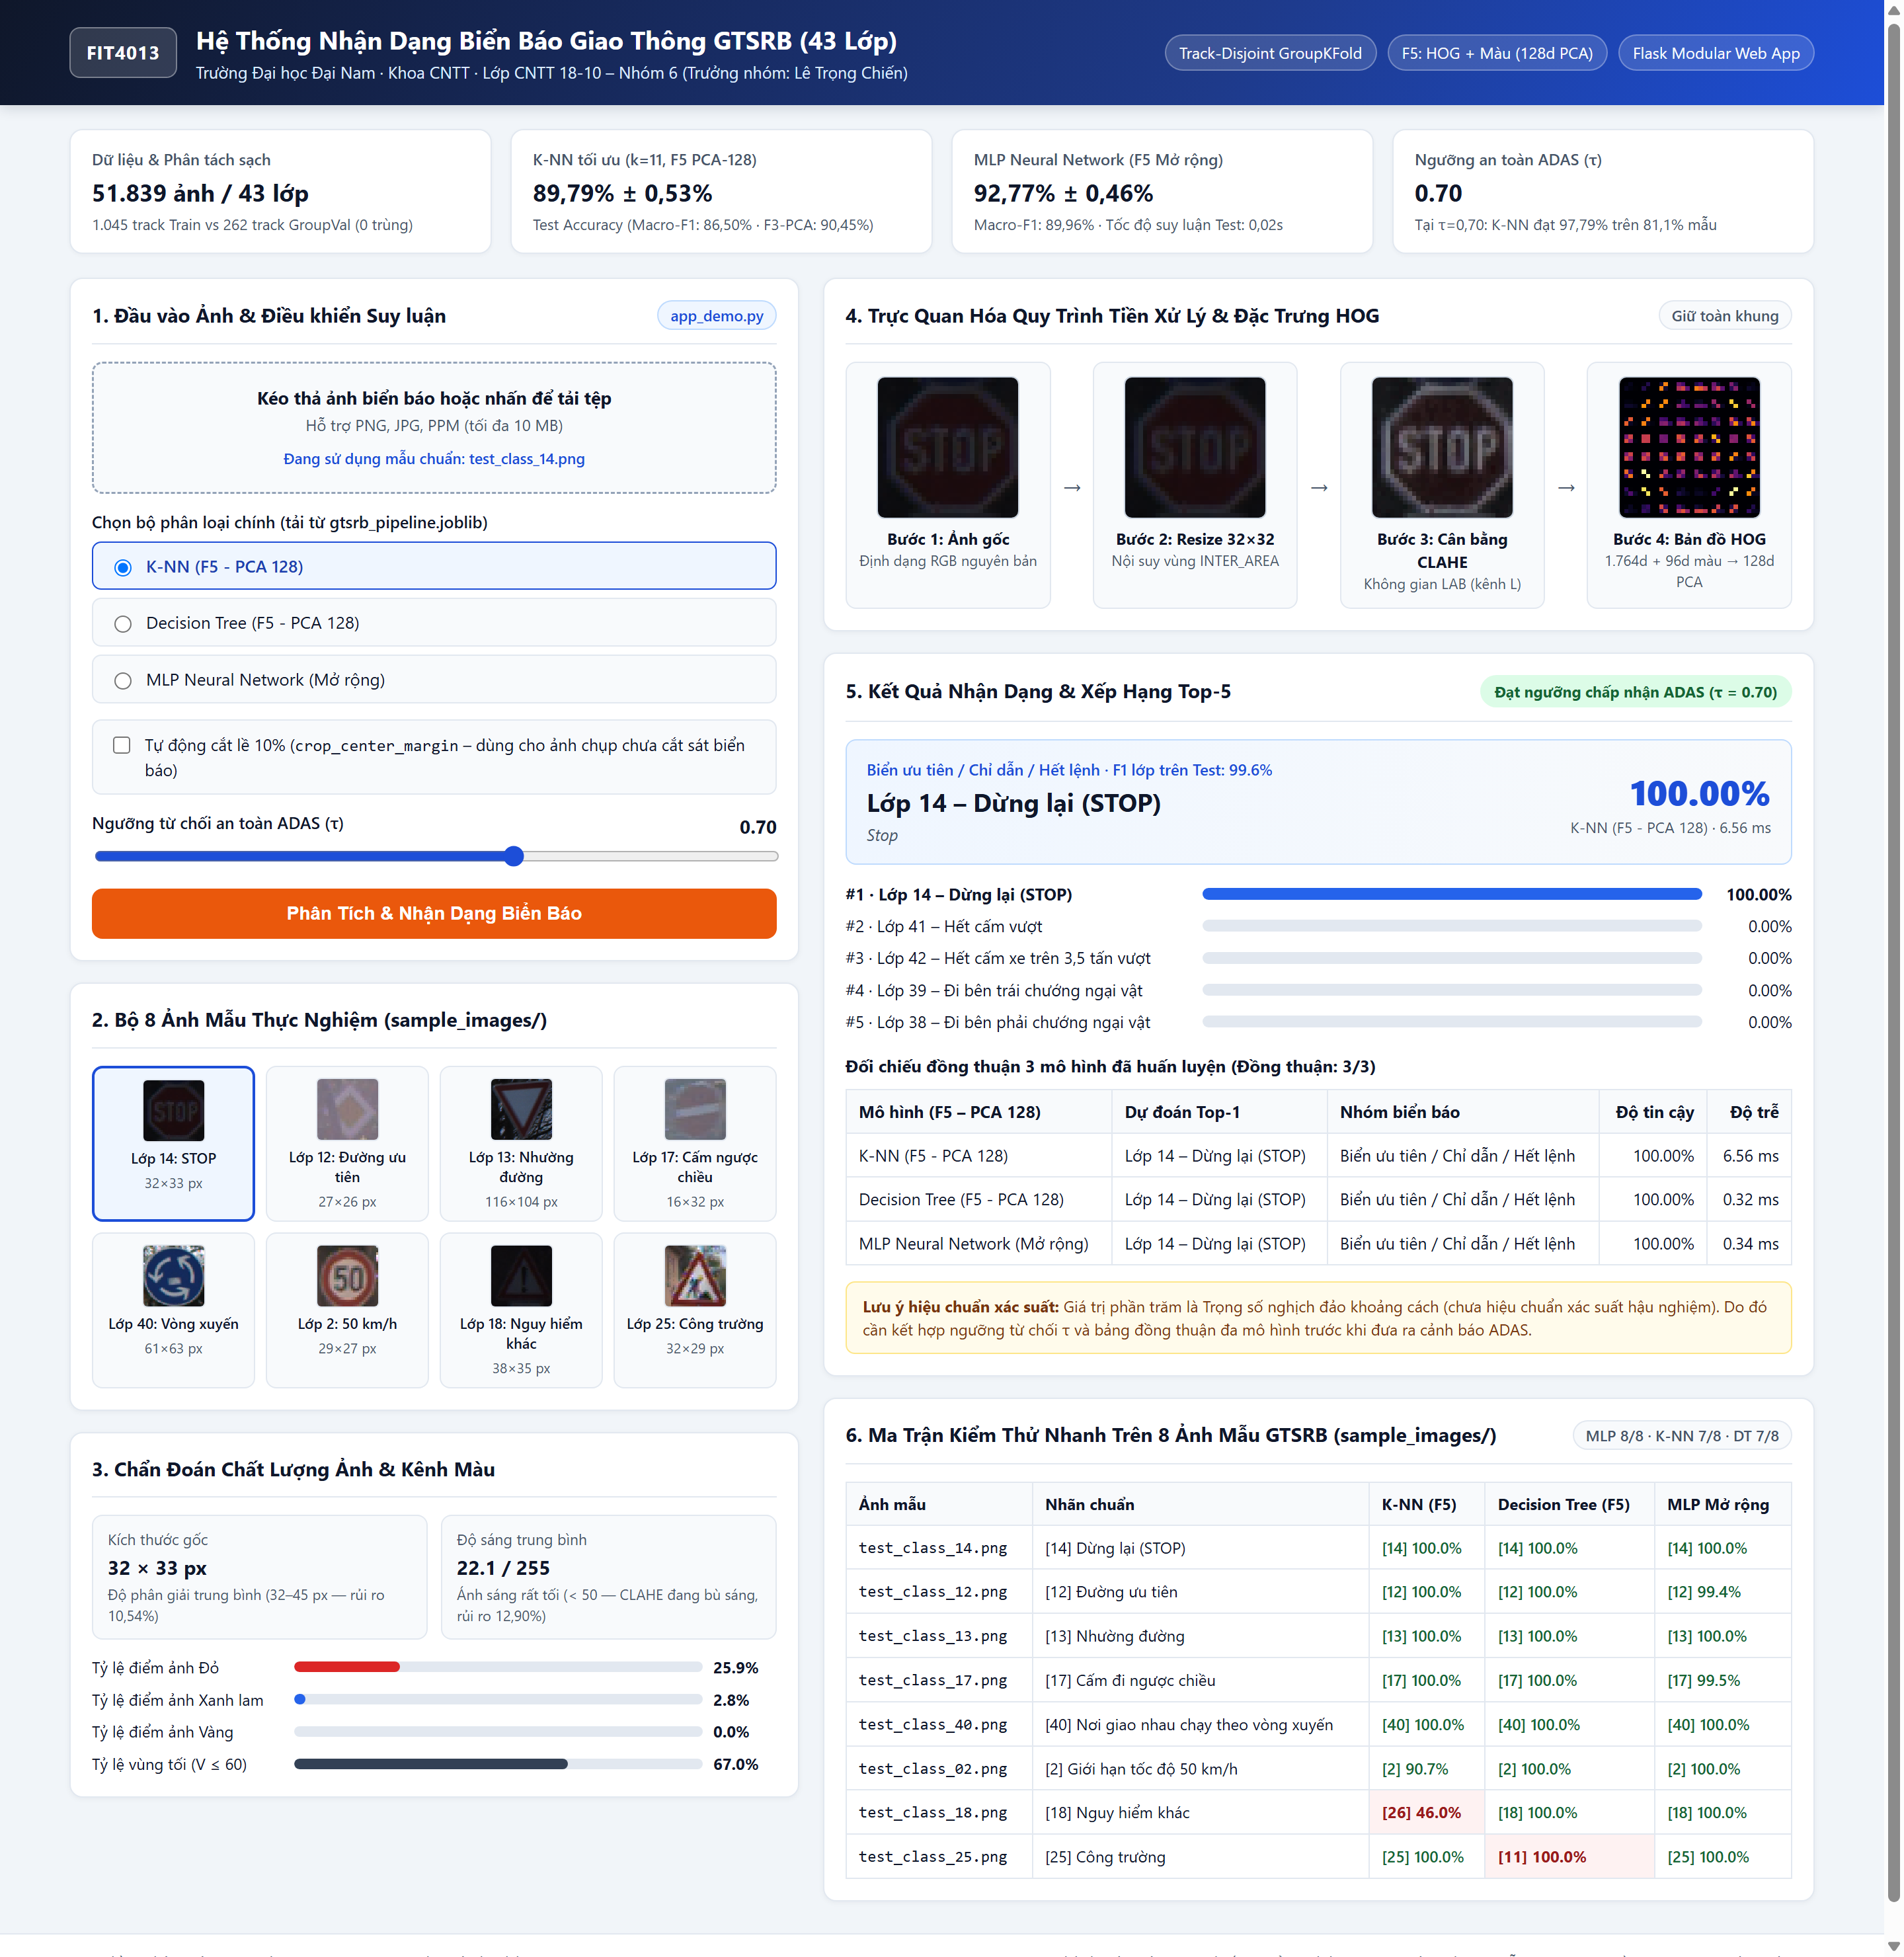
\includegraphics[width=0.68\textwidth]{figures/fig12_demo_app_design.png}
\caption{Thiết kế giao diện Web Dashboard mô-đun bằng Python Flask (gói webapp/ \& app\_demo.py): (trái) Tải ảnh/chọn mẫu, điều chỉnh ngưỡng $\tau$ và chẩn đoán chất lượng ảnh; (phải) Chuỗi trực quan 4 bước, Top-5 dự đoán, đồng thuận K-NN/DT/MLP và ma trận kiểm thử 8 ảnh mẫu.}
\label{fig:demo_design}
\end{figure*}

% ==================== SECTION III ====================
\section{PHÂN TÍCH MÃ NGUỒN VÀ CHỨC NĂNG}

\subsection{Tổ chức kho mã nguồn, môi trường và tái lập thực nghiệm}
Mã nguồn dự án được lưu trữ công khai tại \url{https://github.com/Chieenslee/FIT4013-CNTT-1810-NHOM-6}, đi kèm tệp khai báo thư viện requirements.txt và hướng dẫn tái lập, tổ chức tách bạch thành hai gói mô-đun độc lập là src/ (huấn luyện \& đánh giá) và webapp/ (ứng dụng Web Demo chạy qua lệnh python app\_demo.py):
\begin{itemize}
  \item src/constants.py và src/data\_loader.py: Bảng ánh xạ song ngữ 43 lớp; hàm prepare\_\allowbreak gtsrb\_csvs tổng hợp Train.csv/Test.csv từ dữ liệu tải về và hỗ trợ đọc ảnh an toàn trên đường dẫn Unicode.
  \item src/features.py: Cung cấp các hàm độc lập crop\_roi\_image, apply\_clahe\_rgb, extract\_raw\_gray, extract\_raw\_rgb, extract\_hog\_features và extract\_hog\_\allowbreak color\_features xuất vector kiểu float32 dùng chung cho cả pipeline huấn luyện và tầng dịch vụ Web.
  \item src/pipeline.py: Điều phối phân tách StratifiedGroupKFold theo extract\_track\_ids, tiền xử lý chống rò rỉ (prepare\_\allowbreak scaled\_split), quét lưới GroupVal, đánh giá một lượt tập Test kèm Bootstrap 95\% CI và McNemar, xuất tệp kết quả JSON/CSV, gtsrb\_\allowbreak pipeline.joblib và các biểu đồ PNG.
  \item Gói ứng dụng Web webapp/ và app\_demo.py: Phân lớp rõ ràng gồm webapp/config.py (tham số \& danh mục biển báo), webapp/services/ (model\_\allowbreak registry.py, image\_\allowbreak processor.py, predictor.py), webapp/routes/ (views.py, api.py), giao diện tách file (templates/base.html, templates/index.html, static/css/main.css, static/js/app.js) và điểm khởi chạy gọn nhẹ app\_demo.py.
  \item notebooks/\allowbreak FIT4013\_Nhom6\_\allowbreak DeTai6\_GTSRB\_Colab.ipynb: Sổ tay 8 bước tự động tải trực tiếp 3 tệp nén GTSRB từ máy chủ gốc ERDA, kiểm tra độ sạch, chạy toàn bộ quy trình thực nghiệm và lưu kết quả minh chứng thực thi trên Google Colab.
\end{itemize}

Thực nghiệm được chuẩn hóa trên môi trường phần cứng CPU phổ thông của Google Colab (Google Colab CPU (2 vCPU Intel Xeon, 12.7 GB RAM)) với bộ thư viện Python 3.13.7, NumPy 2.4.4, Pandas 2.3.3, scikit-learn 1.8.0, scikit-image 0.26.0, OpenCV 4.13.0. Tệp requirements.txt quy định phiên bản tối thiểu (numpy $\ge 1.24$, pandas $\ge 2.0$, scikit-learn $\ge 1.3$, opencv-python $\ge 4.8$, scikit-image $\ge 0.21$, joblib $\ge 1.3$, flask $\ge 3.0$).

% ==================== SECTION IV ====================
\section{THỬ NGHIỆM VÀ KẾT QUẢ}

\subsection{Thí nghiệm 1: Đánh giá tách bạch 8 tầng đặc trưng (F0--F5)}
Bảng~\ref{tab:exp1} trình bày đầy đủ hiệu năng của cả 3 thuật toán bắt buộc (K-NN k=5 Euclidean, Decision Tree max\_depth=20 Gini, và Gaussian Naive Bayes) qua 8 phương án biểu diễn đặc trưng. Bốn quy luật thực nghiệm rõ rệt rút ra gồm:
\begin{enumerate}
  \item Tác động của bước cắt ROI (F0 $\rightarrow$ F1): Loại bỏ hậu cảnh ngoài ROI nâng K-NN Test từ 33,55\% lên 50,59\% (+17,04 điểm \%), DT từ 50,22\% lên 56,48\% và GNB từ 9,51\% lên 14,18\%.
  \item Tại sao Decision Tree vượt K-NN trên pixel thô (F0--F2) rồi đảo ngược trên F3--F5: Trên không gian pixel thô, khoảng cách Euclidean của K-NN cộng dồn sai số điểm ảnh do dịch chuyển 2--3 px hoặc đổi bóng đổ trên cả 1.024--3.072 chiều, khiến K-NN chỉ đạt 50,59\% (F1) và 52,89\% (F2). Ngược lại, Decision Tree chọn lọc một số vị trí pixel đặc trưng mang độ lợi thông tin cao ở tâm và viền biển báo nên thắng K-NN trên F0--F2 (50,22\%, 56,48\%, 57,55\%). Khi chuyển sang HOG (F3), tương quan hình học cục bộ giúp K-NN nhảy vọt thêm +39,27 điểm \% lên 89,86\% (Macro-F1 87,00\%), trong khi DT bị giới hạn bởi lát cắt trục tọa độ nên dừng ở 72,05\%.
  \item Vai trò thật của Đặc trưng màu sắc (F3 $\rightarrow$ F4 và F3-PCA $\rightarrow$ F5): Với K-NN, việc ghép thêm 96 chiều màu ở F4 khiến Test Accuracy giảm nhẹ từ 89,86\% xuống 89,34\% (Macro-F1 từ 87,00\% xuống 86,03\%, McNemar p = 0,0050), và trên không gian PCA 128 chiều F3-PCA (90,02\%) cũng cao hơn F5 (89,18\%). Nguyên nhân là StandardScaler đưa phương sai toàn bộ 96 chiều màu nhạy ánh sáng bằng 1 ngang bằng các cạnh HOG, làm nhiễu phép đo khoảng cách láng giềng. Ngược lại, Decision Tree (chọn lọc ngưỡng từng kênh riêng biệt) tăng từ 72,05\% lên 72,32\%, và GNB tăng từ 81,01\% lên 81,37\%.
  \item Vai trò của CLAHE (F4 Không CLAHE $\rightarrow$ F4): Cân bằng sáng CLAHE giúp K-NN cải thiện +0,92 điểm \% (từ 88,42\% lên 89,34\%, kiểm định McNemar p = $5{,}68\times 10^{-5}$), còn GNB tăng từ 80,32\% lên 81,37\%. Đồng thời, khi đưa qua PCA 128 chiều (F5), Gaussian Naive Bayes nhảy vọt từ 14,18\% trên pixel thô lên 88,20\% (Macro-F1 85,57\%).
\end{enumerate}

\begin{table*}[!t]
\centering
\caption{Thí nghiệm 1 -- So sánh tách bạch 8 tầng biểu diễn đặc trưng trên cả 3 thuật toán cốt lõi (K-NN k=5, DT depth=20, GNB)}
\label{tab:exp1}
\footnotesize
\resizebox{\textwidth}{!}{%
\begin{tabular}{@{}l c c c c c c c@{}}
\toprule
\textbf{Biểu diễn đặc trưng} & \textbf{Chiều} & \textbf{K-NN GV} & \textbf{K-NN Test} & \textbf{K-NN F1} & \textbf{DT Test} & \textbf{GNB Test} & \textbf{GNB F1} \\
\midrule
F0: No-ROI Raw Grayscale (1024) & 1024 & 33,98\% & 33,55\% & 28,39\% & 50,22\% & 9,51\% & 10,65\% \\
F1: ROI Raw Grayscale - Baseline (1024) & 1024 & 50,84\% & 50,59\% & 43,76\% & 56,48\% & 14,18\% & 15,23\% \\
F2: ROI Raw RGB (3072) & 3072 & 52,99\% & 52,89\% & 46,35\% & 57,55\% & 17,32\% & 19,25\% \\
F3: ROI + CLAHE + HOG (1764) & 1764 & 92,30\% & 89,86\% & 87,00\% & 72,05\% & 81,01\% & 80,80\% \\
F3-PCA: ROI + CLAHE + HOG + PCA (128) & 128 & 92,06\% & 90,02\% & 87,23\% & 68,58\% & 88,37\% & 85,47\% \\
F4 (Không CLAHE): ROI + HOG + Color (1860) & 1860 & 91,50\% & 88,42\% & 85,04\% & 73,87\% & 80,32\% & 79,13\% \\
F4: ROI + CLAHE + HOG + Color (1860) & 1860 & 91,92\% & 89,34\% & 86,03\% & 72,32\% & 81,37\% & 80,41\% \\
F5: ROI + CLAHE + HOG + Color + PCA (128) & 128 & 91,42\% & 89,18\% & 86,05\% & 68,04\% & 88,20\% & 85,57\% \\
\bottomrule
\end{tabular}%
}
\end{table*}

\subsection{Thí nghiệm 2 \& 3: Tinh chỉnh K-NN (30 cấu hình) và DT (12 cấu hình) trên GroupVal}
Tuân thủ nghiêm ngặt kỷ luật không xem tập Test khi chọn tham số, Bảng~\ref{tab:exp23} và Hình~\ref{fig:hp_tuning} tổng hợp kết quả lưới đầy đủ $5\times 2\times 3 = 30$ cấu hình K-NN và 12 cấu hình Decision Tree đánh giá hoàn toàn trên GroupVal (262 track, 7.860 ảnh). Trên K-NN (F5), hàm trọng số nghịch đảo khoảng cách (distance) luôn vượt trội bỏ phiếu đều (uniform), và độ đo Euclidean đạt đỉnh GroupVal tại k=11 (distance) với 92,24\% Accuracy (88,94\% Macro-F1), nhỉnh nhẹ so với Manhattan (92,19\%) và cao hơn Cosine ở mọi mức k $\ge$ 3. Với Decision Tree, hiện tượng overfitting bộc lộ rõ khi Train đạt 100,00\% tại depth=20 nhưng GroupVal đạt đỉnh tại criterion=entropy, max\_depth=15 (70,13\% Accuracy, 62,43\% Macro-F1) rồi suy giảm nhẹ từ depth $\ge$ 20. Hai cấu hình tối ưu trên GroupVal được chốt cố định để đánh giá một lần cuối trên Test.

\begin{table*}[!t]
\centering
\caption{Thí nghiệm 2 \& 3 -- Kết quả tinh chỉnh siêu tham số K-NN và Decision Tree đánh giá duy nhất trên GroupVal (F5)}
\label{tab:exp23}
\footnotesize
\resizebox{\textwidth}{!}{%
\begin{tabular}{@{}l l c c c c@{}}
\toprule
\textbf{Thuật toán} & \textbf{Cấu hình tiêu biểu} & \textbf{Train Acc} & \textbf{GroupVal Acc} & \textbf{GroupVal Macro-F1} & \textbf{GroupVal Pred (s)} \\
\midrule
K-NN & k=1, uniform, euclidean & -- & 89,81\% & 86,81\% & 1,04 \\
K-NN & k=3, distance, euclidean & -- & 90,66\% & 87,55\% & 1,05 \\
K-NN & k=3, distance, manhattan & -- & 90,69\% & 87,67\% & 10,06 \\
K-NN & k=3, distance, cosine & -- & 90,42\% & 87,08\% & 2,89 \\
K-NN & k=5, uniform, euclidean & -- & 91,32\% & 88,02\% & 1,00 \\
K-NN & k=7, distance, euclidean & -- & 91,81\% & 88,54\% & 0,97 \\
K-NN & k=7, distance, manhattan & -- & 91,87\% & 88,75\% & 10,05 \\
K-NN & k=7, distance, cosine & -- & 91,46\% & 87,83\% & 2,94 \\
K-NN & k=11, uniform, euclidean & -- & 92,09\% & 88,70\% & 1,10 \\
K-NN & k=11, distance, euclidean (Tối ưu GroupVal) & -- & 92,24\% & 88,94\% & 1,08 \\
K-NN & k=11, distance, manhattan & -- & 92,19\% & 88,92\% & 10,19 \\
K-NN & k=11, distance, cosine & -- & 91,95\% & 88,23\% & 3,04 \\
\midrule
Decision Tree & gini, max\_depth=5 & 29,14\% & 29,99\% & 13,20\% & 0,00 \\
Decision Tree & gini, max\_depth=10 & 61,73\% & 57,96\% & 40,28\% & 0,00 \\
Decision Tree & gini, max\_depth=15 & 84,38\% & 67,40\% & 57,64\% & 0,00 \\
Decision Tree & gini, max\_depth=20 & 96,64\% & 69,20\% & 60,14\% & 0,00 \\
Decision Tree & gini, max\_depth=None & 100,00\% & 68,66\% & 59,77\% & 0,00 \\
Decision Tree & entropy, max\_depth=5 & 51,03\% & 48,61\% & 29,48\% & 0,00 \\
Decision Tree & entropy, max\_depth=10 & 80,25\% & 68,52\% & 60,75\% & 0,00 \\
Decision Tree & entropy, max\_depth=15 (Tối ưu GroupVal) & 98,40\% & 70,13\% & 62,43\% & 0,00 \\
Decision Tree & entropy, max\_depth=20 & 100,00\% & 69,80\% & 62,02\% & 0,00 \\
Decision Tree & entropy, max\_depth=None & 100,00\% & 69,80\% & 62,02\% & 0,00 \\
\bottomrule
\end{tabular}%
}
\end{table*}

\begin{figure*}[!t]
\centering
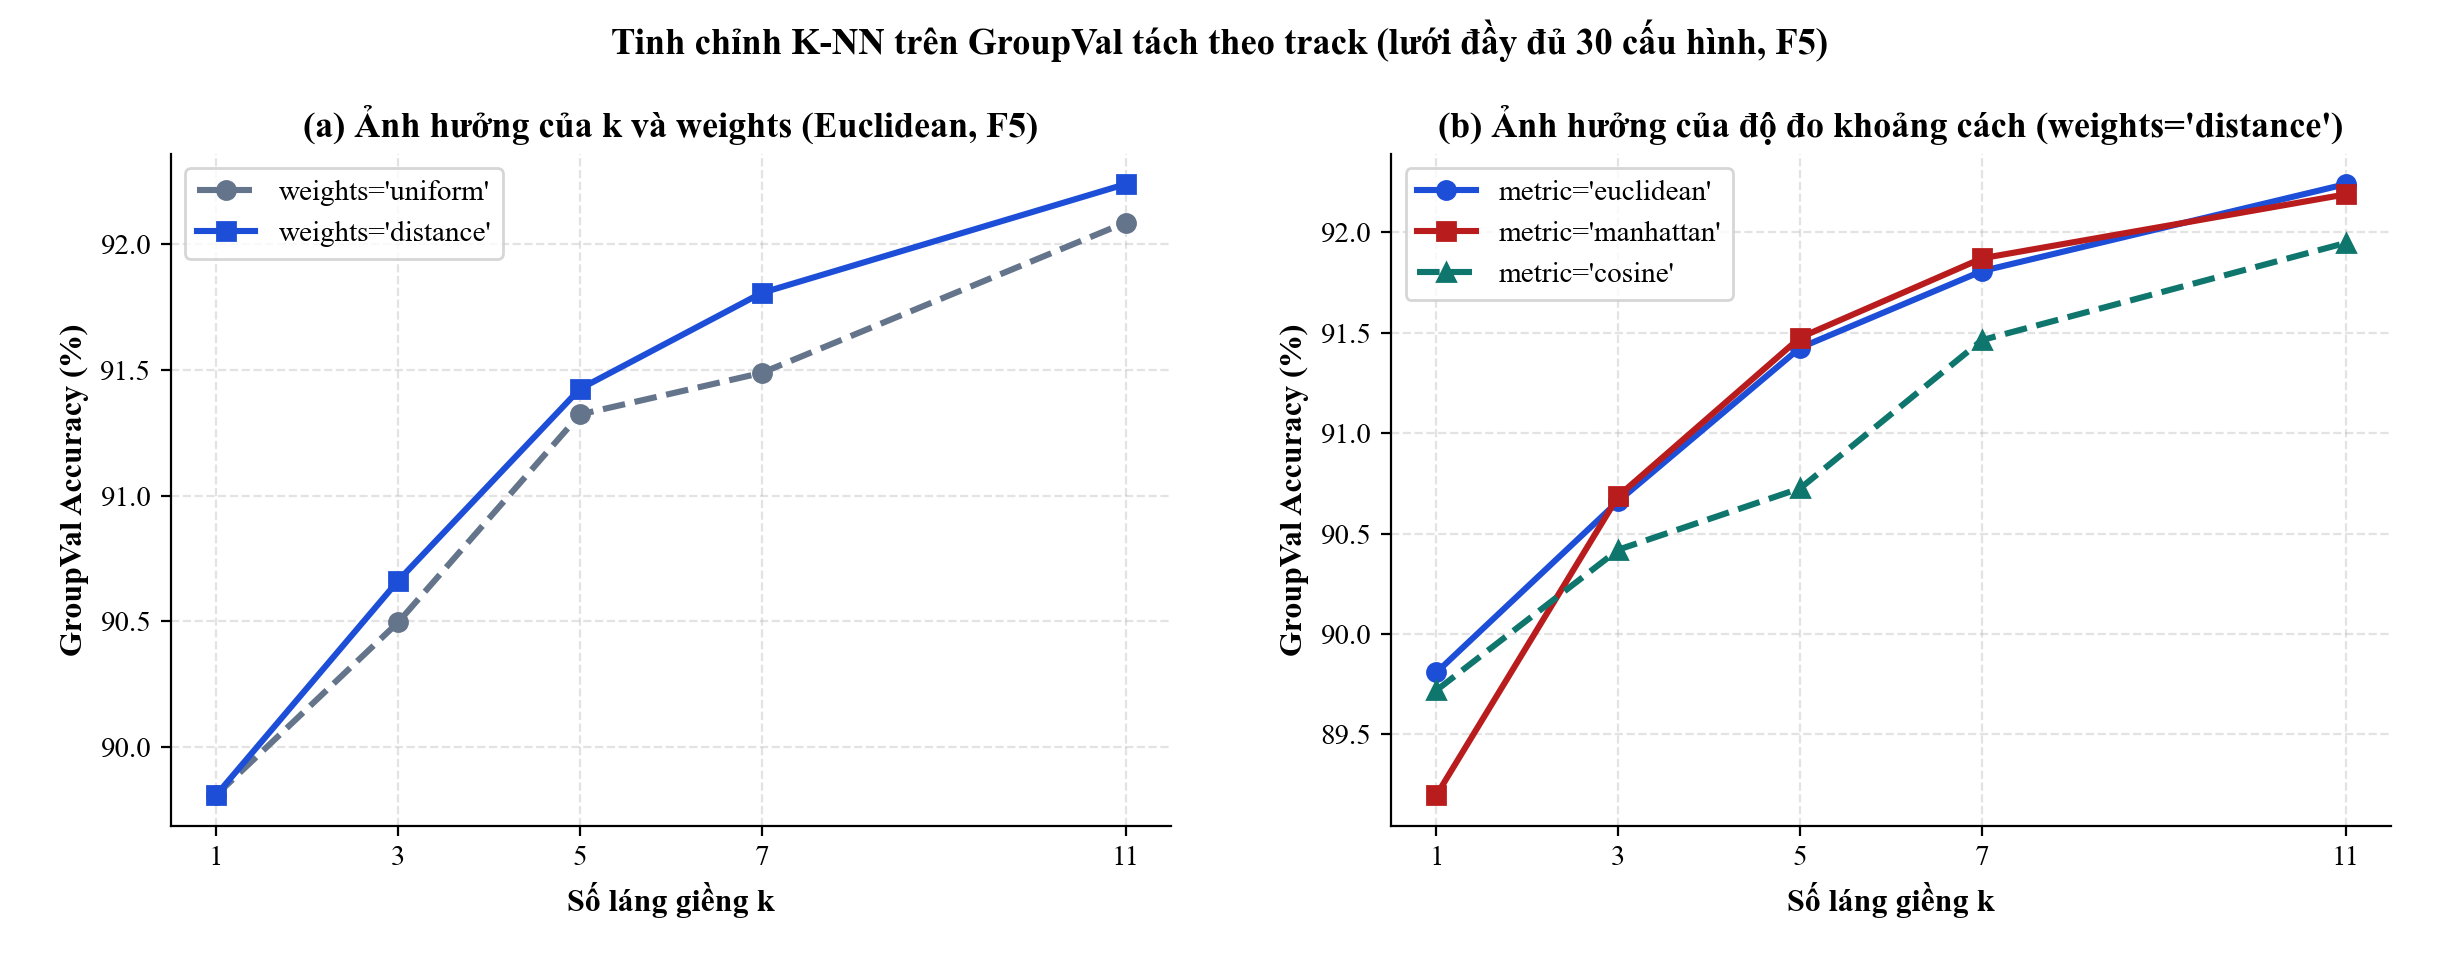
\includegraphics[width=0.49\textwidth]{figures/fig5_knn_hyperparams.png}\hfill
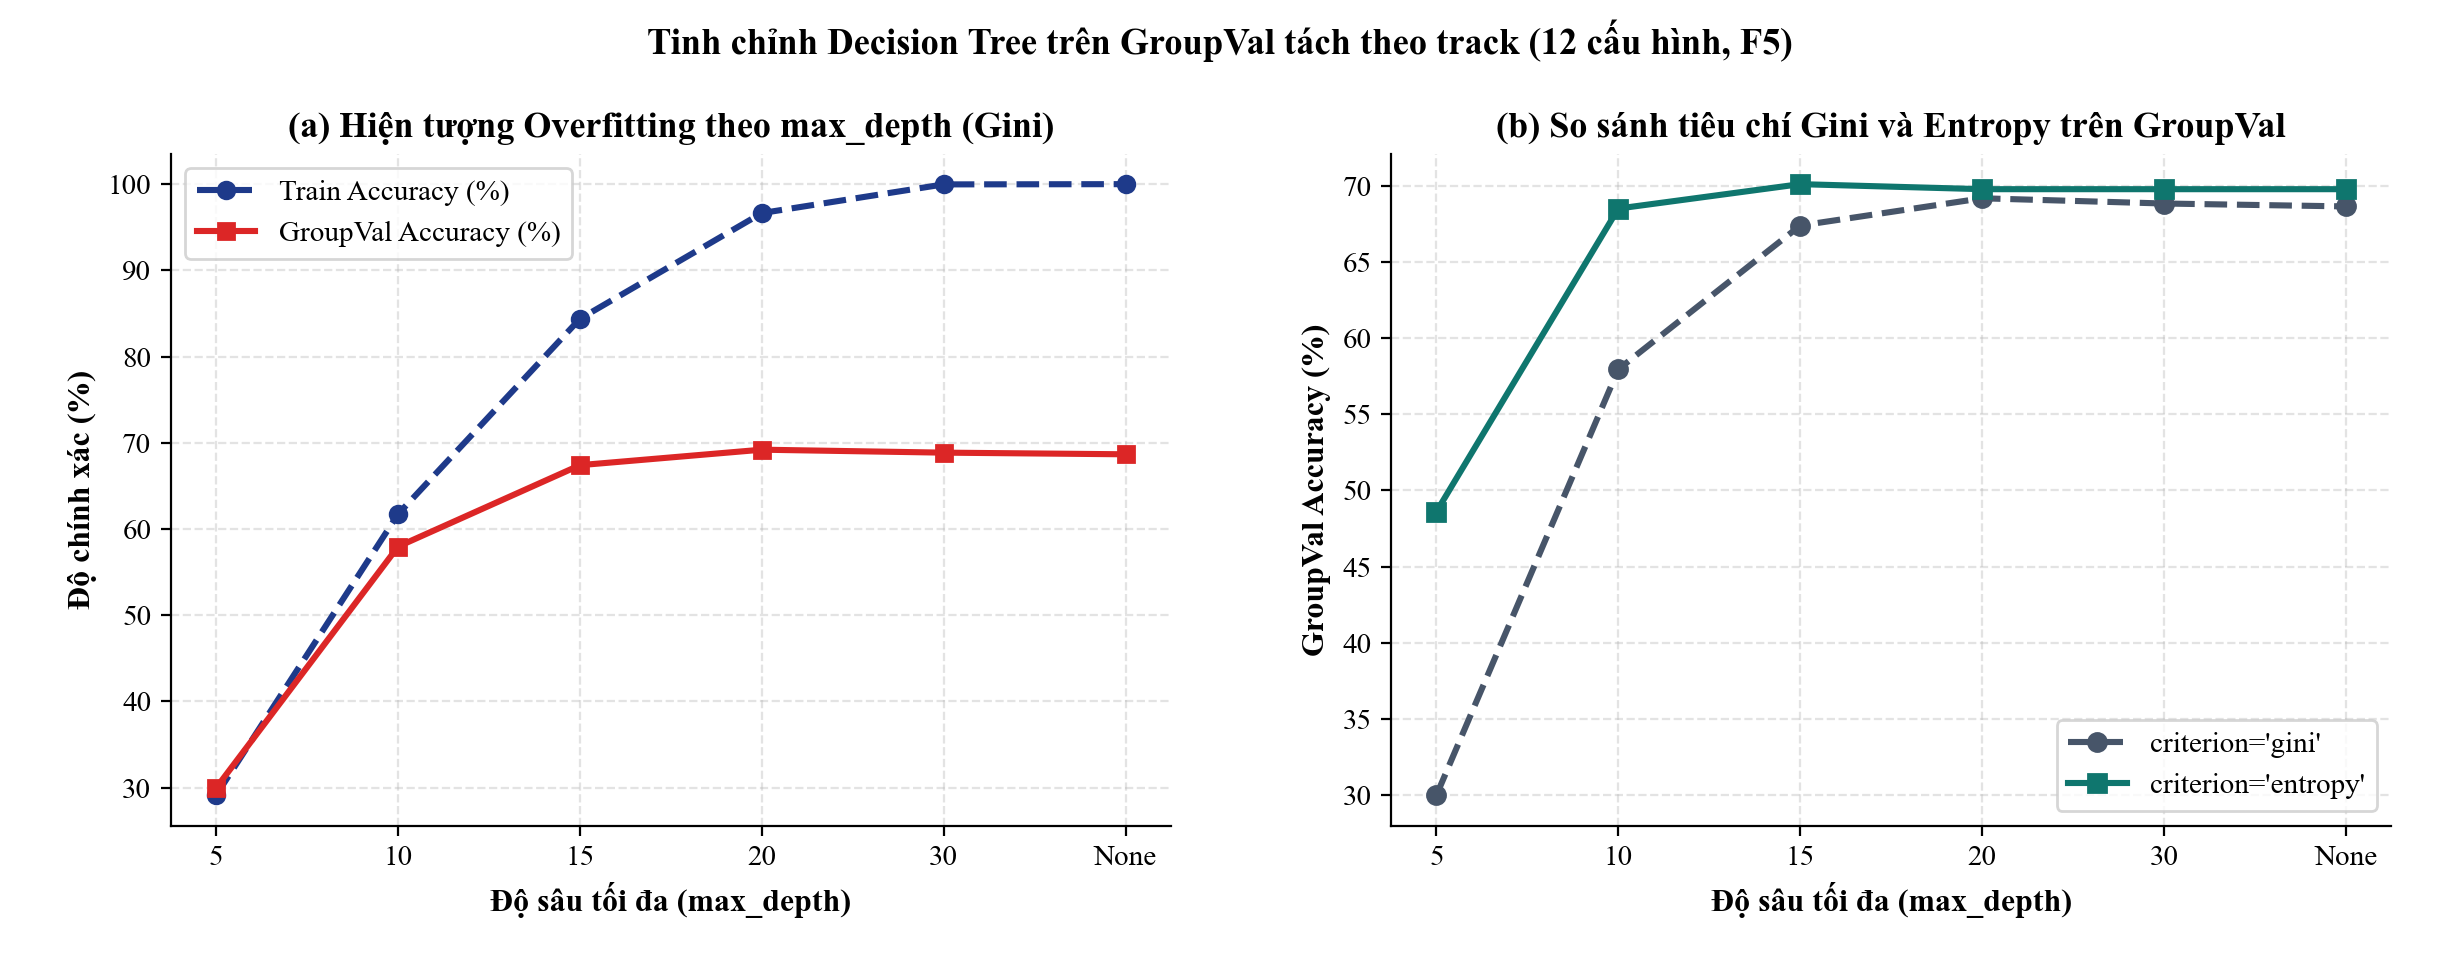
\includegraphics[width=0.49\textwidth]{figures/fig6_dt_hyperparams.png}
\caption{Đường cong tinh chỉnh siêu tham số đánh giá trên GroupVal tách theo track: (trái) K-NN 30 cấu hình; (phải) Decision Tree 12 cấu hình.}
\label{fig:hp_tuning}
\end{figure*}

\subsection{Thí nghiệm 4: Phân tích số chiều PCA xác định (Full SVD) trên GroupVal}
Sử dụng PCA(n\_components=512, svd\_solver=full) cho kết quả hoàn toàn tất định (d=128 khớp chính xác 64,74\% phương sai với cấu hình F5 độc lập). Bảng~\ref{tab:exp4} và Hình~\ref{fig:pca} (đầu dò K-NN k=11 Cosine trên GroupVal) cho thấy tại d=128, mô hình giữ lại 64,74\% phương sai và đạt 91,95\% GroupVal Accuracy (gần tương đương mức nguyên bản 1.860 chiều ở 91,96\%) trong khi thời gian suy luận giảm từ 6,27s xuống 3,03s. Mức d=256 đạt GroupVal cao nhất ở đầu dò Cosine (92,42\%, 78,70\% phương sai), còn d=128 cân bằng tốt giữa chi phí lưu trữ vector (gấp 14,5 lần nhỏ hơn 1.860 chiều) và độ chính xác.

\begin{table}[!t]
\centering
\caption{Thí nghiệm 4 -- Quét chiều PCA trên GroupVal (K-NN k=11, Cosine)}
\label{tab:exp4}
\footnotesize
\setlength{\tabcolsep}{4pt}
\resizebox{\columnwidth}{!}{%
\begin{tabular}{@{}l c c c c@{}}
\toprule
\textbf{Số chiều d} & \textbf{Phương sai} & \textbf{GroupVal Acc} & \textbf{GV Macro-F1} & \textbf{Pred (s)} \\
\midrule
32 & 45,87\% & 86,01\% & 80,22\% & 3,23 \\
64 & 54,28\% & 90,03\% & 85,86\% & 3,08 \\
128 & 64,74\% & 91,95\% & 88,23\% & 3,03 \\
256 & 78,70\% & 92,42\% & 89,11\% & 3,22 \\
512 & 95,34\% & 91,95\% & 88,78\% & 3,61 \\
1860 (Gốc F4) & 100,00\% & 91,96\% & 89,01\% & 6,27 \\
\bottomrule
\end{tabular}%
}
\end{table}

\begin{figure}[!t]
\centering
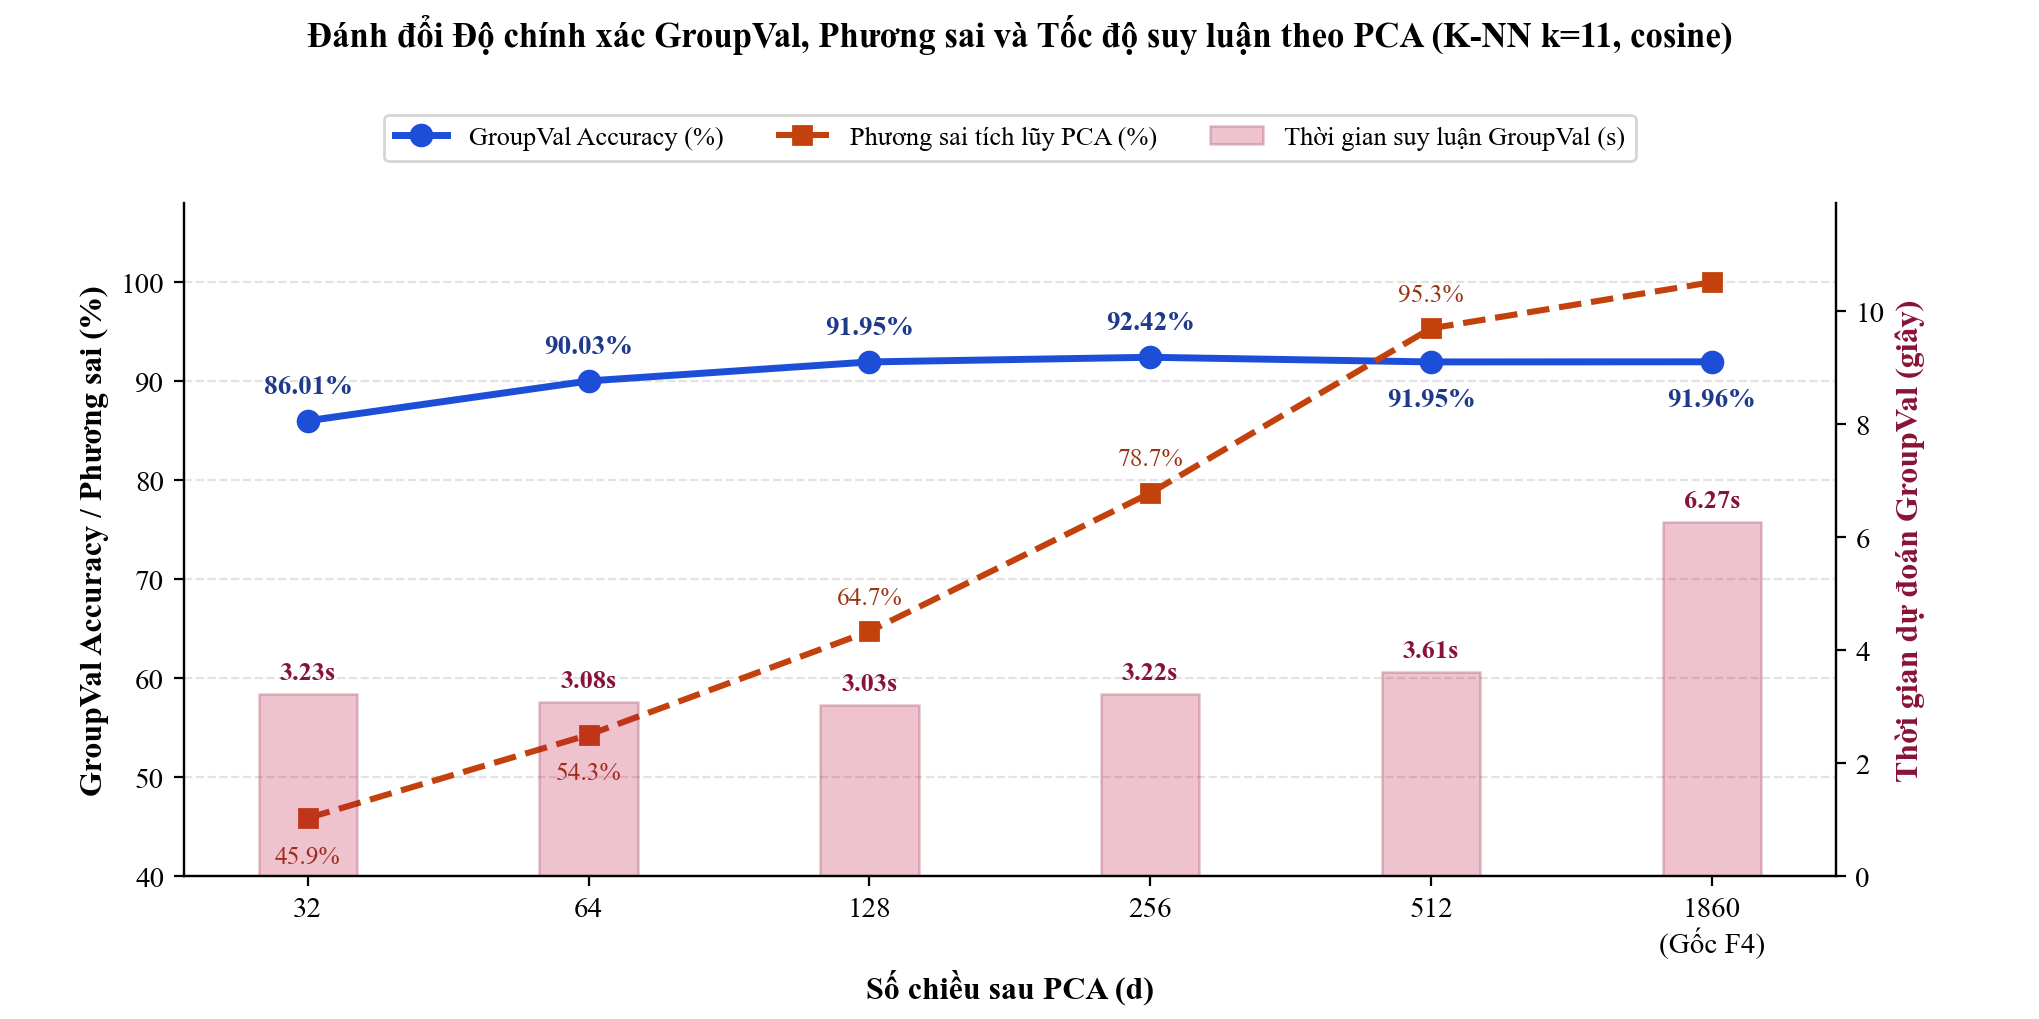
\includegraphics[width=\columnwidth]{figures/fig7_pca_analysis.png}
\caption{Đánh đổi GroupVal Accuracy, phương sai tích lũy và thời gian dự đoán theo số chiều PCA (svd\_solver=full).}
\label{fig:pca}
\end{figure}

\subsection{Thí nghiệm 5: Đánh giá trên tập Test khóa, kiểm định 95\% CI và Demo}
Bảng~\ref{tab:exp5} và Hình~\ref{fig:comp} trình bày kết quả đánh giá cuối cùng một lần trên 12.630 ảnh Test độc lập kèm khoảng tin cậy Bootstrap 95\% (1.000 lần lấy mẫu lại) cho toàn bộ 11 cấu hình tách biệt hoàn toàn:
\begin{enumerate}
  \item Trong các thuật toán bắt buộc của học phần trên F5, K-NN tối ưu (k=11, distance, Euclidean) đạt 89,79\% ($\pm$ 0,53\%) Test Accuracy và 86,50\% ($\pm$ 0,85\%) Macro-F1, cao hơn Gaussian Naive Bayes (88,20\%, Macro-F1 85,57\%, kiểm định McNemar $\chi^2 = 32,14$, p = $1{,}43\times 10^{-8}$) và Decision Tree (69,07\%, Macro-F1 59,45\%). Đổi lại, GNB suy luận nhanh gần 5 lần so với K-NN Euclidean (0,35s so với 1,72s) và không cần lưu trữ ma trận 31.349 vector mẫu.
  \item Trên không gian HOG thuần nén PCA (K-NN F3-PCA, k=11 Euclidean), mô hình đạt 90,45\% Test Accuracy và 87,48\% Macro-F1, cao hơn có ý nghĩa thống kê so với K-NN F5 (89,79\%, McNemar p = 0,0004). Việc loại bỏ PCA ở K-NN F4 (1.860 chiều) chỉ đạt 89,81\% tương đương thống kê với K-NN F5 trong khi thời gian dự đoán chậm hơn 10 lần (18,06s so với 1,72s).
  \item Chênh lệch tốc độ giữa K-NN Euclidean (1,72s) và K-NN Manhattan đối chứng (89,95\%, dự đoán 12,01s) bắt nguồn từ cơ chế cài đặt của scikit-learn tối ưu khoảng cách $L_2$ qua phép nhân ma trận BLAS $\|a-b\|_2^2 = \|a\|_2^2 + \|b\|_2^2 - 2a^Tb$, không phải do độ phức tạp tiệm cận thuật toán khác nhau.
  \item Ở phần mở rộng, Random Forest (200 cây) đạt 87,73\% Test Accuracy (Macro-F1 81,79\%), còn mạng MLP đạt hiệu năng cao nhất 92,77\% ($\pm$ 0,46\%) và Macro-F1 89,96\% ($\pm$ 0,75\%) chỉ với 0,02 giây suy luận (McNemar p = $5{,}02\times 10^{-32}$ khi đối chiếu với K-NN F5).
  \item Đối chiếu với mốc tham chiếu trong tài liệu gốc IJCNN 2011 của Stallkamp et al.~\cite{stallkamp2012man}: con người đạt 98,84\%, hệ thống CNN đa tỷ lệ và Committee CNN đạt 98,31\%--99,46\%, còn các hệ thống tuyến tính LDA kết hợp HOG đơn lẻ chuẩn cuộc thi đạt 93,18\%--95,68\% với 1.568--2.916 chiều đặc trưng. Như vậy, kết quả 92,77\% của mạng MLP hai lớp ẩn trên chỉ 128 chiều nén PCA đã tiệm cận mức HOG-LDA gốc với dung lượng vector gọn hơn hơn 12 lần.
\end{enumerate}

\begin{table*}[!t]
\centering
\caption{Thí nghiệm 5 -- Kết quả trên tập Test khóa (12.630 ảnh) kèm khoảng tin cậy Bootstrap 95\% (n=1.000)}
\label{tab:exp5}
\footnotesize
\resizebox{\textwidth}{!}{%
\begin{tabular}{@{}l c c c c c c c@{}}
\toprule
\textbf{Mô hình / Đặc trưng} & \textbf{GroupVal} & \textbf{Test Acc (95\% CI)} & \textbf{Macro-F1 (95\% CI)} & \textbf{Macro-P} & \textbf{Macro-R} & \textbf{Fit (s)} & \textbf{Pred (s)} \\
\midrule
Baseline K-NN (k=5, Raw Gray F1) & 50,84\% & 50,59 $\pm$ 0,87\% & 43,76 $\pm$ 0,98\% & 47,25\% & 42,36\% & 0,07 & 9,75 \\
Baseline Decision Tree (Raw Gray F1) & 59,08\% & 56,48 $\pm$ 0,84\% & 47,07 $\pm$ 1,04\% & 48,68\% & 46,37\% & 66,58 & 0,02 \\
Gaussian Naive Bayes (Raw Gray F1) & 14,95\% & 14,18 $\pm$ 0,58\% & 15,23 $\pm$ 0,72\% & 26,32\% & 18,22\% & 0,23 & 2,85 \\
K-NN F3-PCA (11, euclidean) & 92,79\% & 90,45 $\pm$ 0,49\% & 87,48 $\pm$ 0,80\% & 89,59\% & 86,33\% & 0,01 & 1,66 \\
K-NN tối ưu F5 (k=11, euclidean) & 92,24\% & 89,79 $\pm$ 0,53\% & 86,50 $\pm$ 0,85\% & 88,37\% & 85,43\% & 0,02 & 1,72 \\
K-NN F5 (11, manhattan đối chứng) & 92,19\% & 89,95 $\pm$ 0,54\% & 86,97 $\pm$ 0,87\% & 89,44\% & 85,51\% & 0,01 & 12,01 \\
K-NN F4 không PCA (k=11, euclidean) & 92,58\% & 89,81 $\pm$ 0,53\% & 86,60 $\pm$ 0,77\% & 89,11\% & 85,48\% & 0,09 & 18,06 \\
Decision Tree F5 (depth=15, entropy) & 70,13\% & 69,07 $\pm$ 0,78\% & 59,45 $\pm$ 1,08\% & 60,63\% & 59,13\% & 51,08 & 0,01 \\
Gaussian Naive Bayes (F5) & 91,03\% & 88,20 $\pm$ 0,58\% & 85,57 $\pm$ 0,79\% & 89,42\% & 84,53\% & 0,04 & 0,35 \\
Random Forest (200 trees, F5) & 89,80\% & 87,73 $\pm$ 0,56\% & 81,79 $\pm$ 0,95\% & 90,04\% & 78,72\% & 26,94 & 0,30 \\
MLP Neural Network (F5) & 94,73\% & 92,77 $\pm$ 0,46\% & 89,96 $\pm$ 0,75\% & 92,08\% & 88,64\% & 17,16 & 0,02 \\
\bottomrule
\end{tabular}%
}
\end{table*}

\begin{figure*}[!t]
\centering
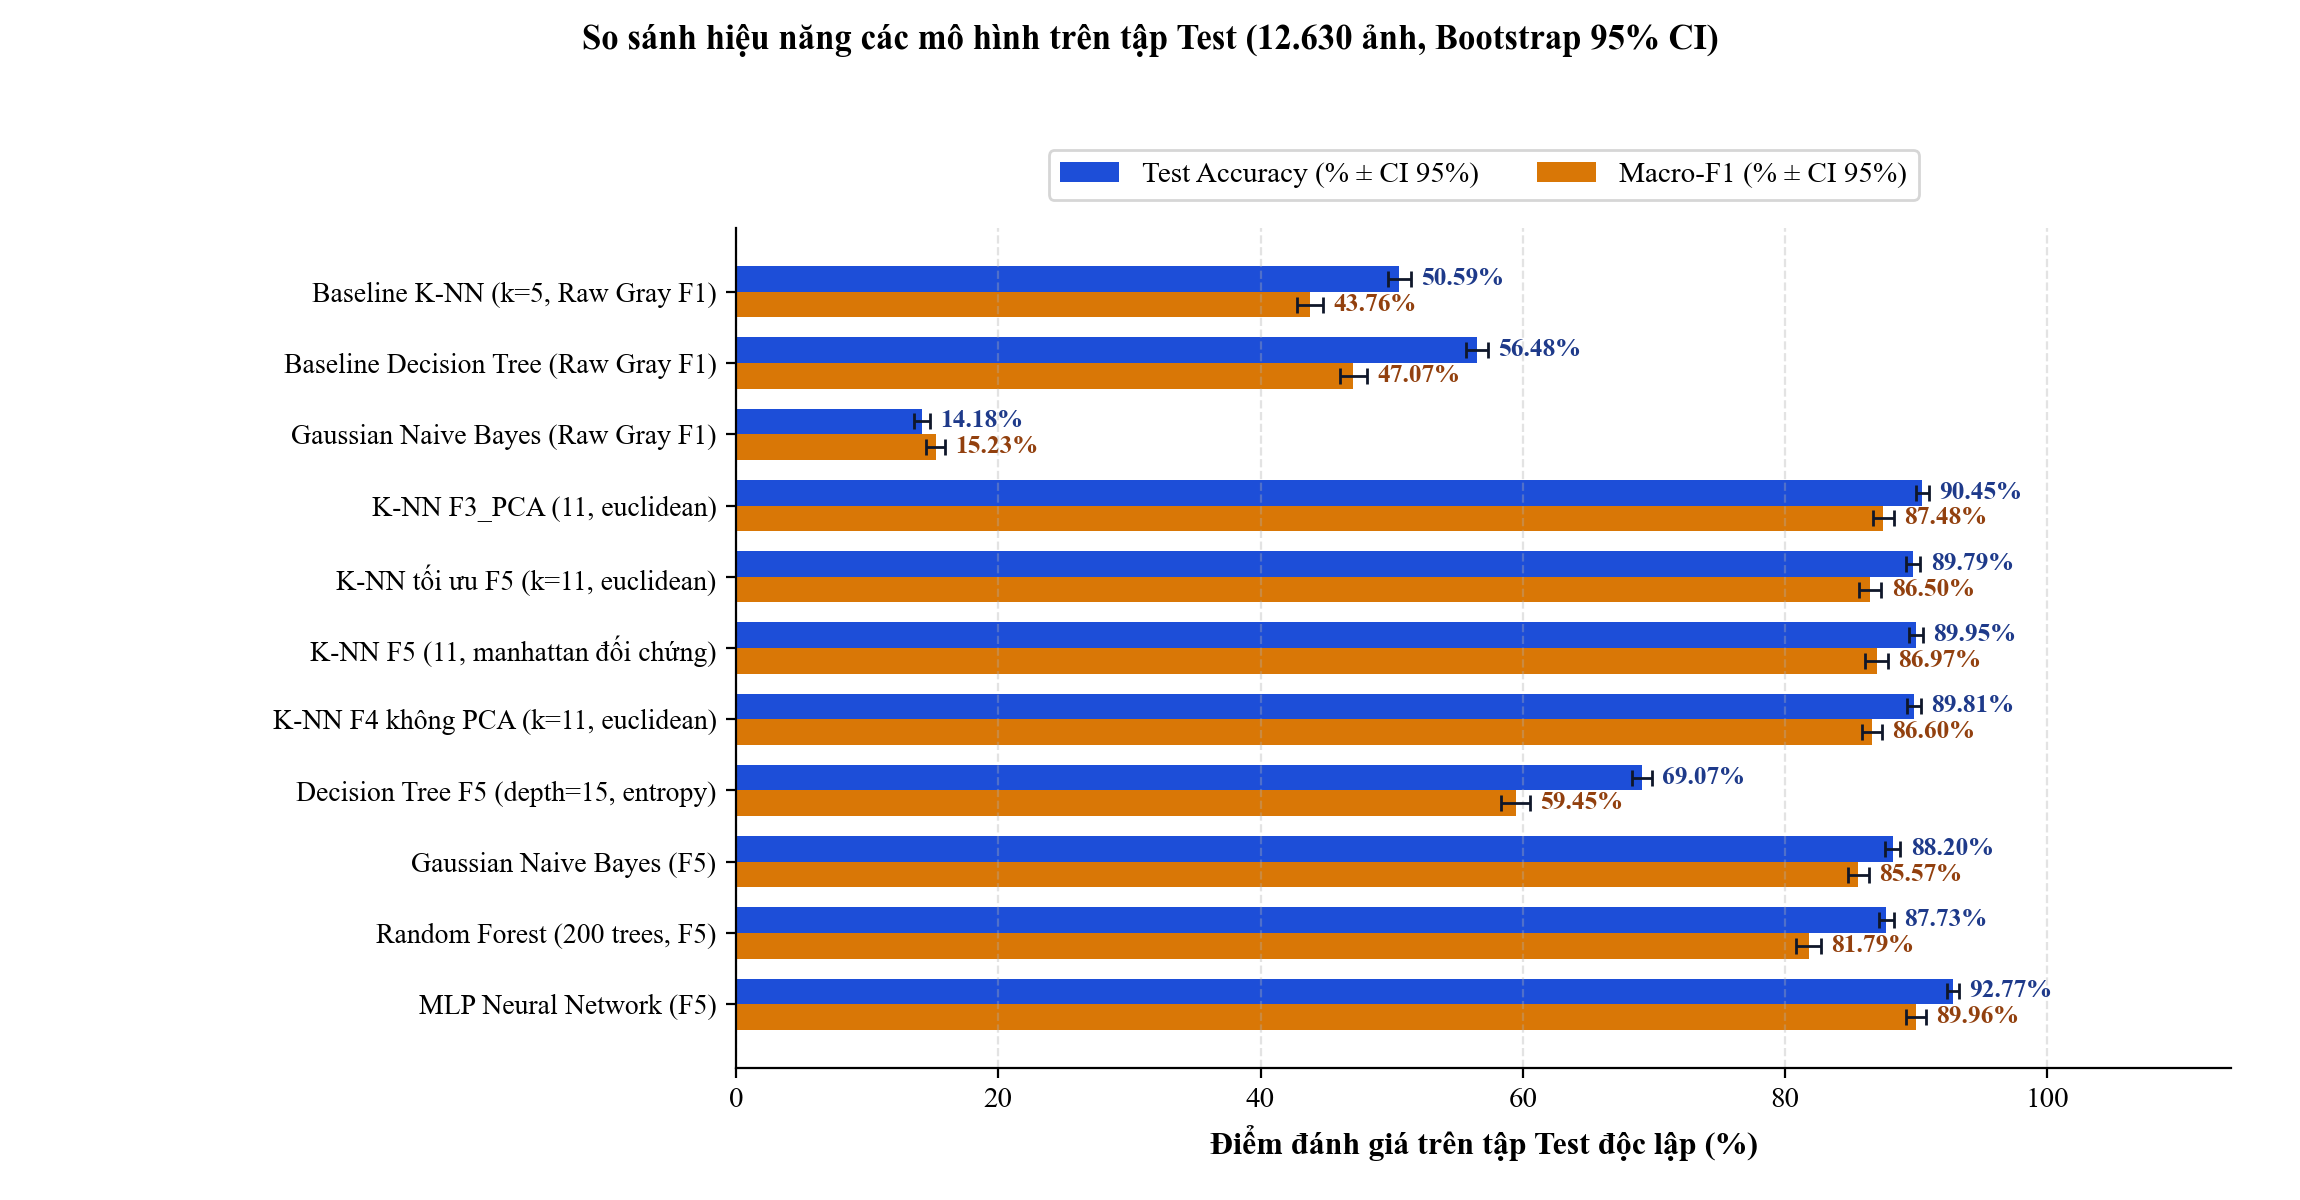
\includegraphics[width=0.66\textwidth]{figures/fig8_model_comparison.png}
\caption{Đối sánh hiệu năng Test Accuracy và Macro-F1 kèm thanh sai số Bootstrap 95\% CI giữa 11 mô hình thực nghiệm.}
\label{fig:comp}
\end{figure*}

Hình~\ref{fig:cm} hiển thị ma trận nhầm lẫn chuẩn hóa $43\times 43$ của K-NN F5 (điểm số đỏ biểu diễn số lượng ảnh nhầm tại các ô ngoài đường chéo $\ge 5\%$). Kiểm thử trực tiếp trên ứng dụng Web Demo (Hình~\ref{fig:demo_design}) với toàn bộ 8 ảnh mẫu thuộc sample\_images/ ghi nhận: MLP dự đoán chính xác 8/8 lớp với độ tin cậy 99,39\%--100,00\% (~0,2--0,6 ms/ảnh); K-NN đạt 7/8 lớp (~4--22 ms/ảnh, riêng mẫu khó test\_class\_18.png K-NN ra Lớp 26 ở mức 45,99\% dưới ngưỡng từ chối $\tau=0{,}70$ và được MLP lẫn Decision Tree đồng thuận sửa đúng thành Lớp 18); Decision Tree đạt 7/8 lớp (~0,2--3 ms/ảnh).

\begin{figure*}[!t]
\centering
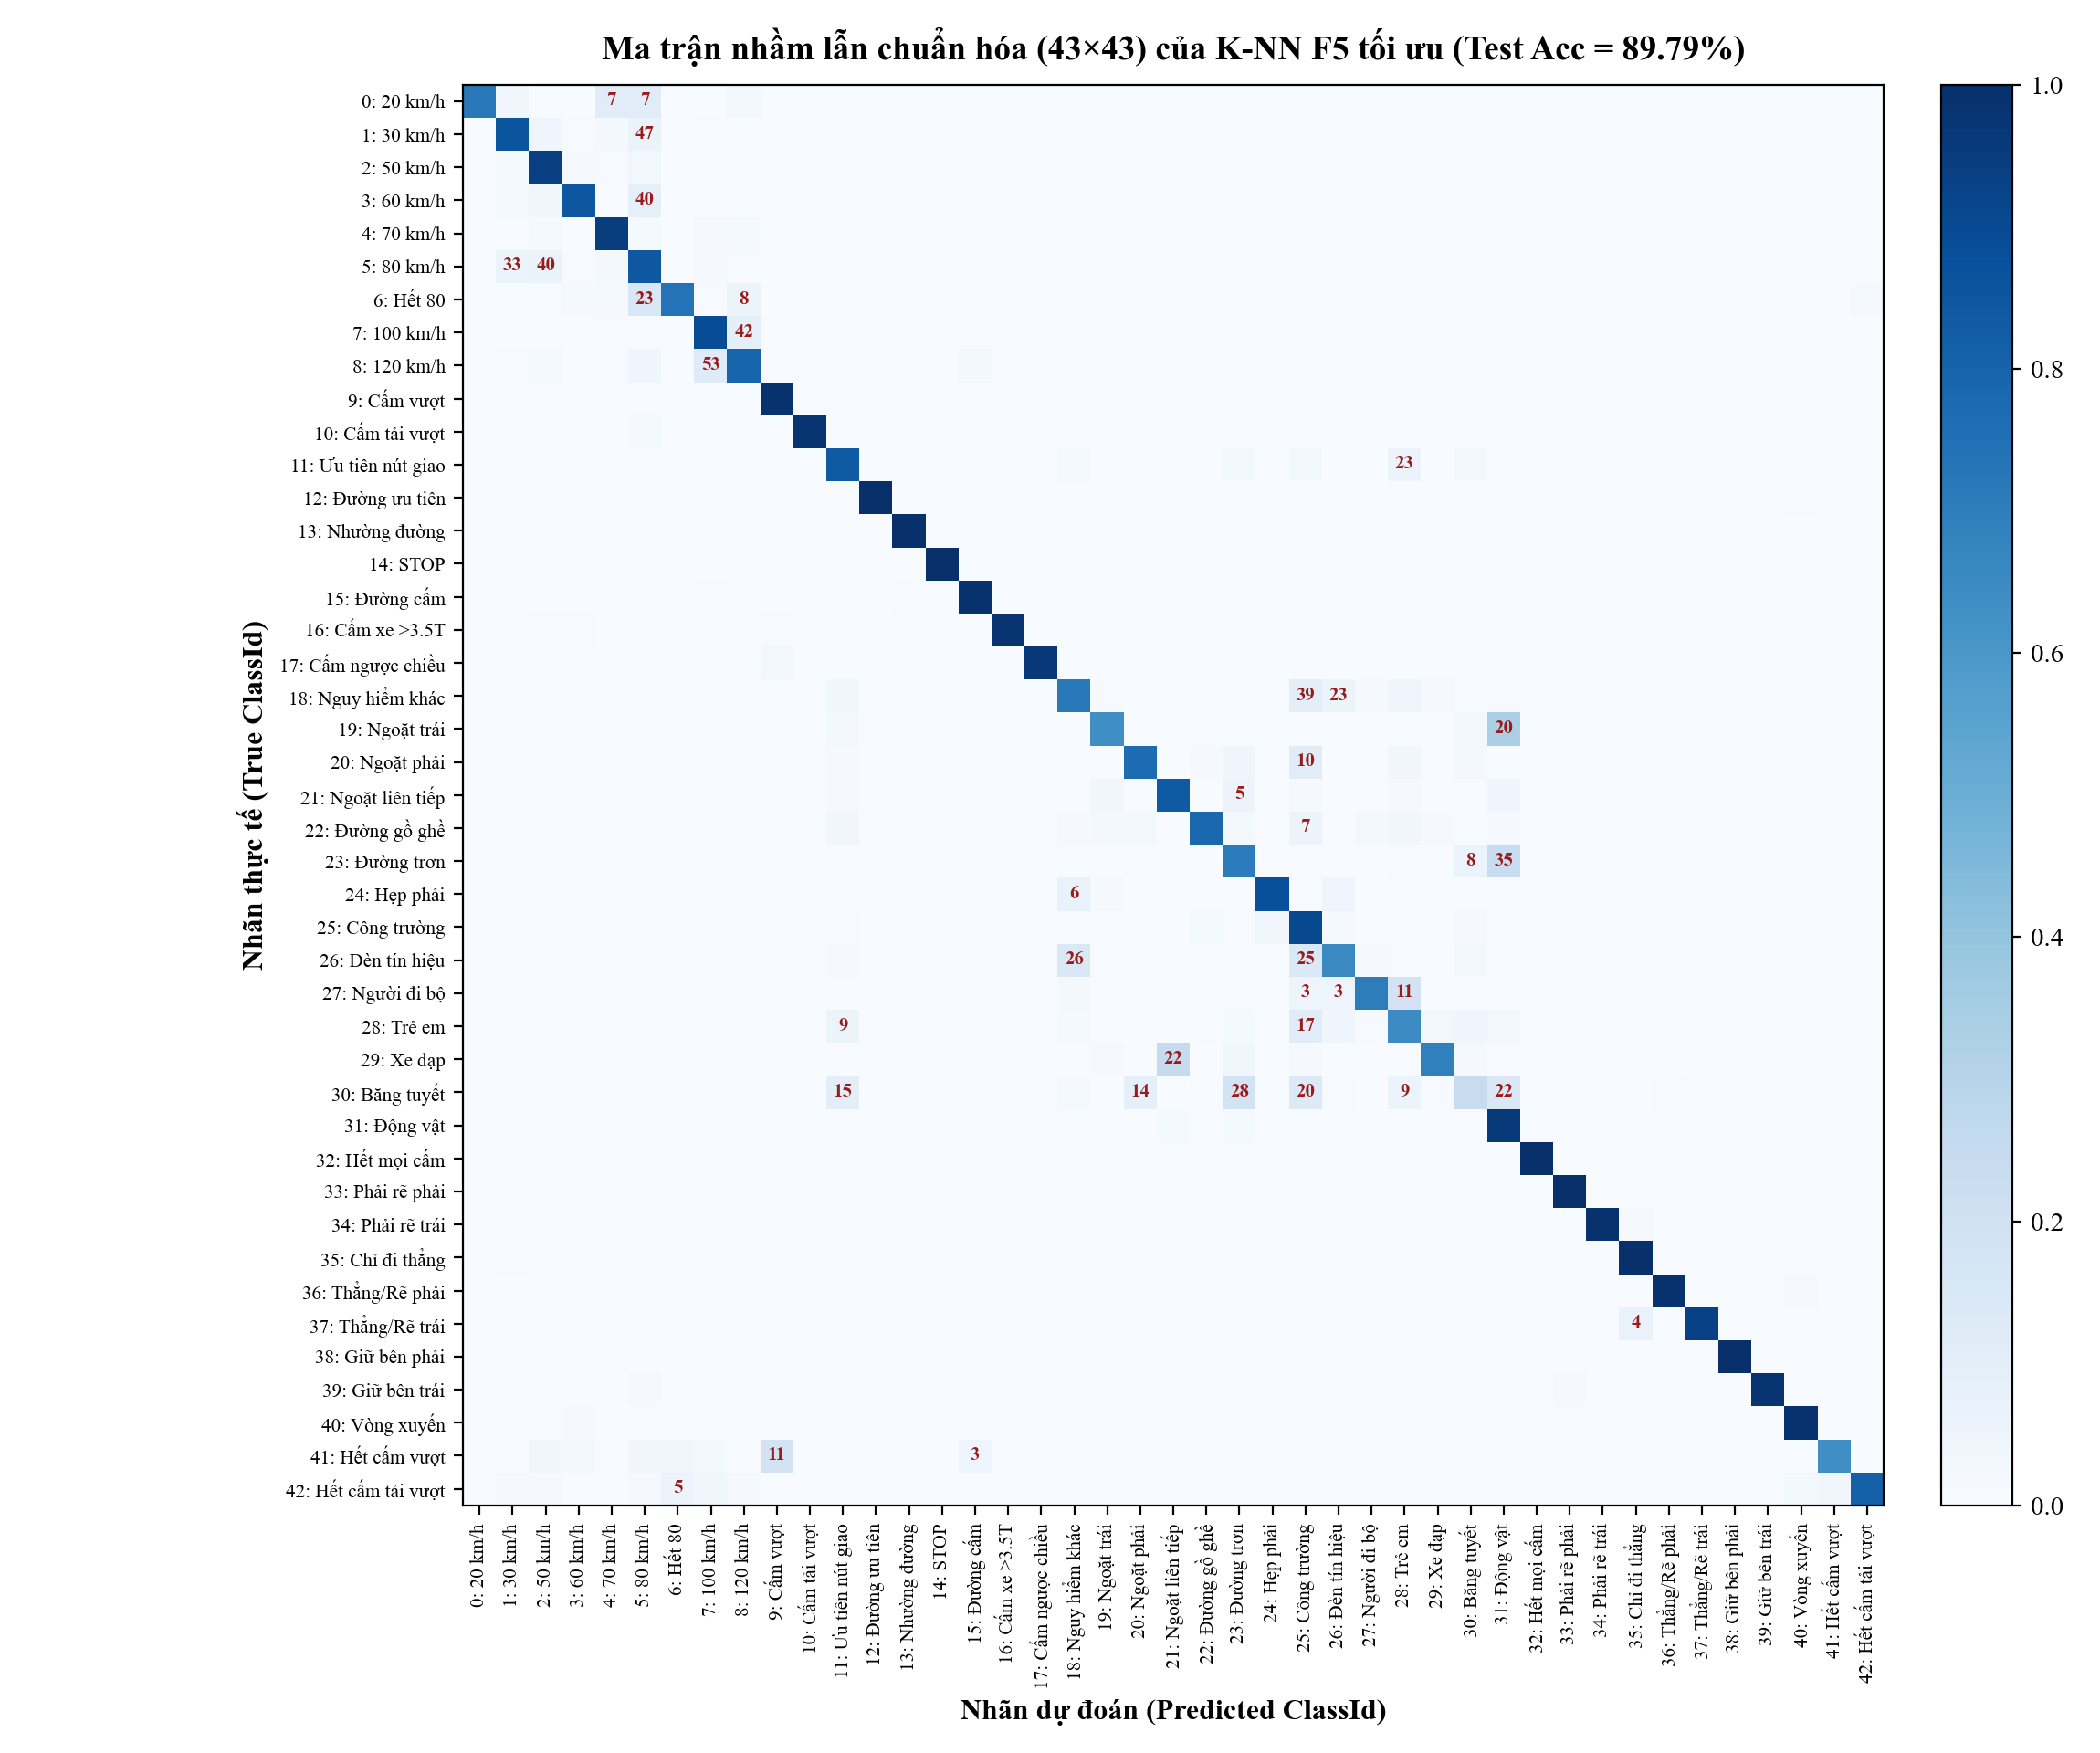
\includegraphics[width=0.55\textwidth]{figures/fig9_confusion_matrix.png}
\caption{Ma trận nhầm lẫn chuẩn hóa $43\times 43$ của K-NN F5 kèm chú thích số lượng ảnh nhầm ngoài đường chéo ($\ge 5\%$).}
\label{fig:cm}
\end{figure*}

% ==================== SECTION V ====================
\section{THẢO LUẬN VÀ SO SÁNH}

\subsection{Lý giải hành vi thuật toán và hạn chế RF/PCA}
\begin{enumerate}
  \item Độ lợi từ bất biến cục bộ HOG: Vector pixel thô đo trực tiếp độ chênh sáng từng điểm ảnh cố định nên rất nhạy với lệch tâm. HOG tổng hợp gradient theo ô $4\times 4$ và chuẩn hóa khối L2-Hys nên ổn định trước dịch chuyển nhỏ và bóng râm cục bộ, giải thích bước tăng +39,27 điểm \% giữa F1 và F3.
  \item Tương tác giữa PCA và các thuật toán: Decision Tree sử dụng lát cắt trực giao theo từng trục tọa độ nên sau phép quay tuyến tính PCA, các ranh giới lớp bị kéo chéo khiến cây đơn lẻ khó xấp xỉ hiệu quả (69,07\%). Với Gaussian Naive Bayes, phép chiếu PCA thực hiện khử tương quan tuyến tính bậc hai thông qua chéo hóa ma trận hiệp phương sai mẫu toàn cục $\Sigma_{\text{global}}$ trên tập huấn luyện, giúp mô hình tiến gần hơn tới giả định các thành phần trực giao dù chưa đảm bảo độc lập có điều kiện hoàn toàn trong từng lớp ($\Sigma_c$ vẫn có thể còn hiệp phương sai chéo). Do mỗi lớp biển báo còn chứa các cụm ánh sáng đa đỉnh (multimodal), bộ phân loại dựa trên khoảng cách K-NN (89,79\%) và mạng phi tuyến MLP (92,77\%) linh hoạt hơn GNB (88,20\%).
  \item Độ lệch Accuracy--Macro Recall ở Random Forest: Bảng~\ref{tab:exp5} ghi nhận Random Forest đạt Test Accuracy 87,73\% nhưng Macro-Recall chỉ đạt 78,72\% (chênh lệch gần 9 điểm \%). Nguyên nhân là cấu hình mặc định class\_weight=None ưu tiên giảm lỗi tạp chất Gini trên các lớp có hàng nghìn mẫu (Lớp 1, 2, 12, 13, 38) và bỏ sót các lớp thiểu số chỉ có 60--150 mẫu kiểm thử.
\end{enumerate}

\subsection{Kiểm chứng lỗi định lượng theo kích thước, độ sáng và Coverage--Accuracy}
Trên tập Test của K-NN (F5), ba lớp đạt F1 cao nhất là Lớp 32 (Hết mọi lệnh cấm, F1 = 100,0\%), Lớp 13 (Nhường đường, 99,9\%) và Lớp 38 (Đi bên phải chướng ngại vật, 99,9\%); ba lớp khó nhất là Lớp 30 (Cảnh báo băng tuyết, F1 = 31,3\%), Lớp 28 (Trẻ em qua đường, 60,8\%) và Lớp 23 (Đường trơn trượt, 66,0\%). Bảng~\ref{tab:errors} thống kê Top 10 cặp nhầm lẫn hai chiều phổ biến nhất (trong đó cặp 120 km/h $\leftrightarrow$ 100 km/h chiếm 95 ảnh gồm 53 chiều 120 $\rightarrow$ 100 và 42 chiều 100 $\rightarrow$ 120). Hình~\ref{fig:err_gallery} minh họa 8 mẫu lỗi trực quan điển hình (00196.ppm (28$\times$27 px: [8] $\rightarrow$ [7]); 00076.ppm (45$\times$51 px: [1] $\rightarrow$ [5]); 00087.ppm (36$\times$41 px: [7] $\rightarrow$ [8]); 00266.ppm (28$\times$28 px: [5] $\rightarrow$ [2]); 00760.ppm (47$\times$48 px: [3] $\rightarrow$ [5]); 00198.ppm (44$\times$40 px: [18] $\rightarrow$ [25]); 00012.ppm (79$\times$73 px: [23] $\rightarrow$ [31]); 00213.ppm (51$\times$49 px: [5] $\rightarrow$ [1])).

\begin{table*}[!t]
\centering
\caption{Top 10 cặp lớp nhầm lẫn hai chiều (K-NN F5 trên 12.630 ảnh Test)}
\label{tab:errors}
\footnotesize
\setlength{\tabcolsep}{7pt}
\begin{tabular}{@{}c l r r r@{}}
\toprule
\textbf{\#} & \textbf{Cặp lớp (A $\leftrightarrow$ B)} & \textbf{A$\rightarrow$B} & \textbf{B$\rightarrow$A} & \textbf{Tổng} \\
\midrule
1 & [8] 120 km/h $\leftrightarrow$ [7] 100 km/h & 53 & 42 & 95 \\
2 & [1] 30 km/h $\leftrightarrow$ [5] 80 km/h & 47 & 33 & 80 \\
3 & [5] 80 km/h $\leftrightarrow$ [2] 50 km/h & 40 & 22 & 62 \\
4 & [26] Đèn tín hiệu $\leftrightarrow$ [18] Nguy hiểm khác & 26 & 23 & 49 \\
5 & [1] 30 km/h $\leftrightarrow$ [2] 50 km/h & 32 & 11 & 43 \\
6 & [3] 60 km/h $\leftrightarrow$ [5] 80 km/h & 40 & 3 & 43 \\
7 & [18] Nguy hiểm khác $\leftrightarrow$ [25] Công trường & 39 & 3 & 42 \\
8 & [23] Đường trơn $\leftrightarrow$ [31] Động vật & 35 & 4 & 39 \\
9 & [30] Băng tuyết $\leftrightarrow$ [23] Đường trơn & 28 & 8 & 36 \\
10 & [26] Đèn tín hiệu $\leftrightarrow$ [25] Công trường & 25 & 7 & 32 \\
\bottomrule
\end{tabular}
\end{table*}

\begin{figure*}[!t]
\centering
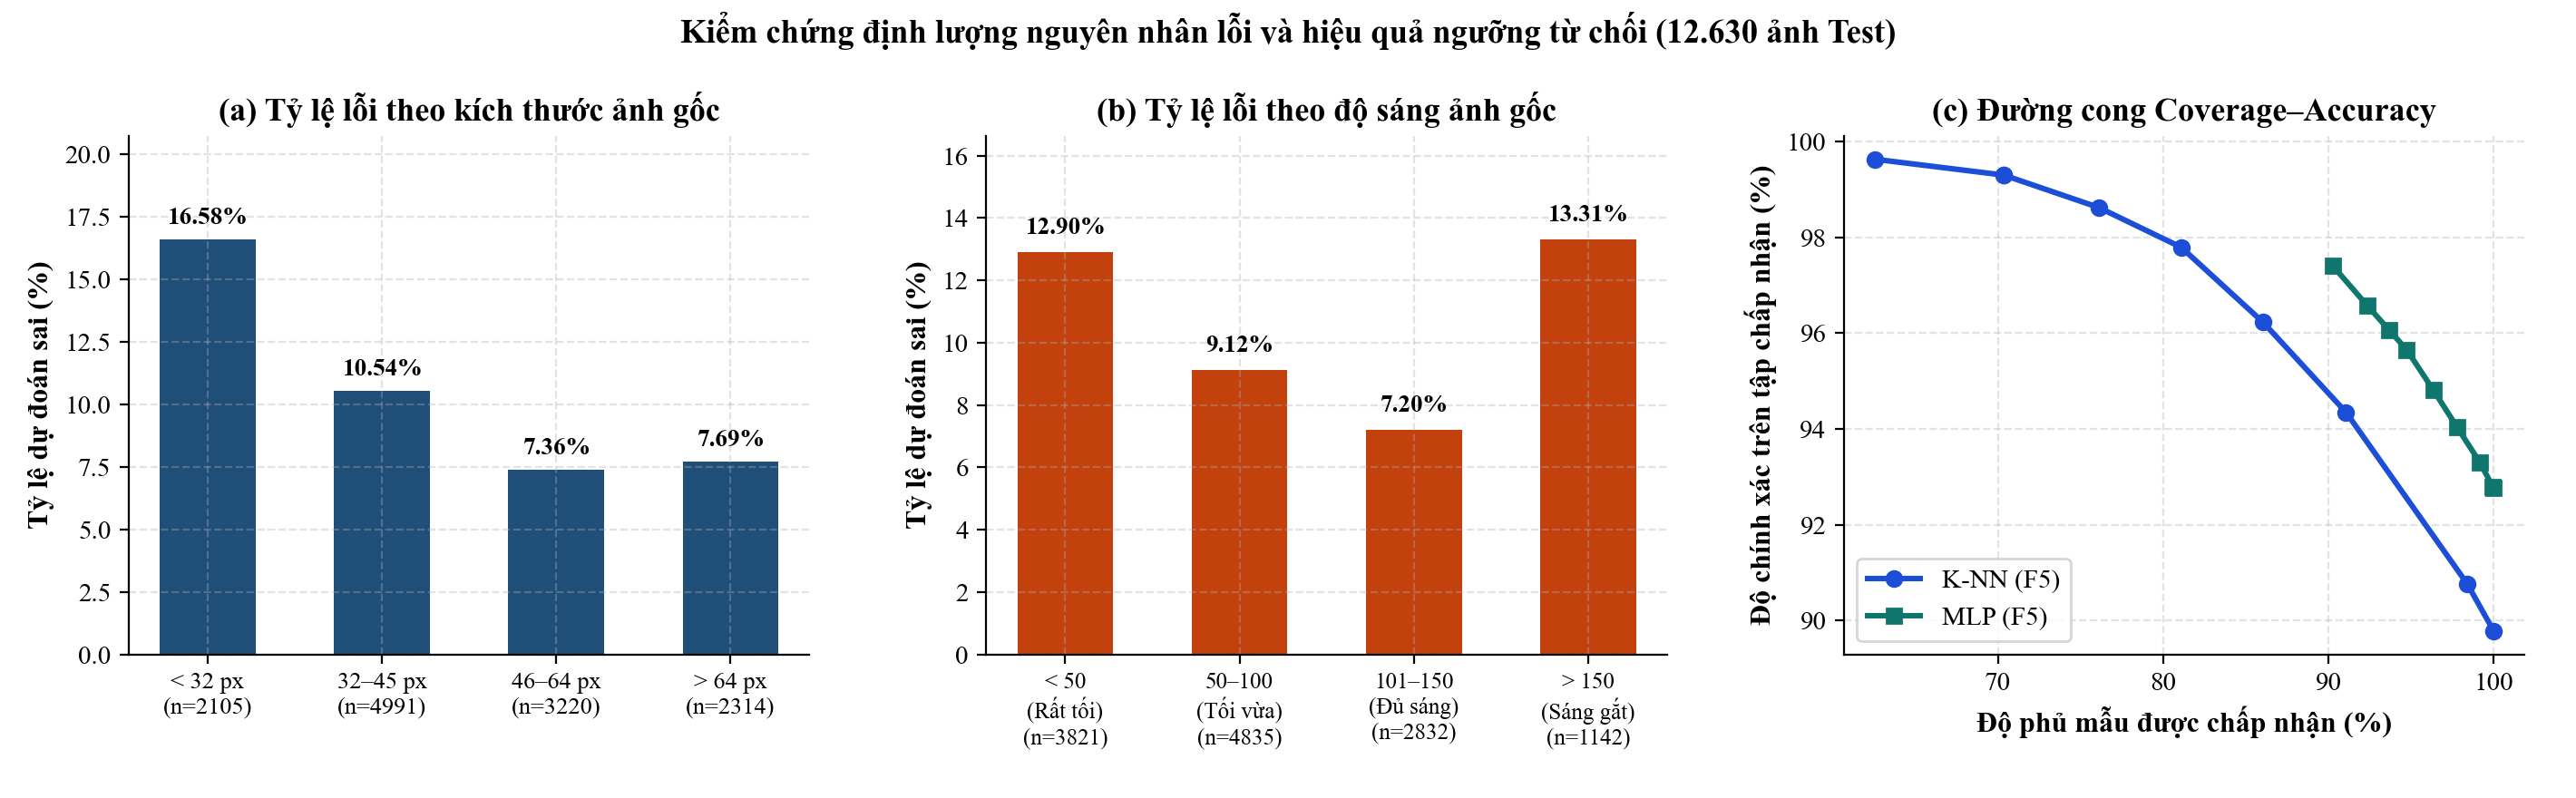
\includegraphics[width=0.76\textwidth]{figures/fig11_error_diagnostics.png}
\caption{Kiểm chứng định lượng nguyên nhân lỗi trên toàn bộ 12.630 ảnh Test: (a) Tỷ lệ lỗi theo kích thước ảnh gốc; (b) Tỷ lệ lỗi theo độ sáng trung bình; (c) Đường cong Coverage--Accuracy của K-NN F5 và MLP F5.}
\label{fig:err_diag}
\end{figure*}

\begin{figure*}[!t]
\centering
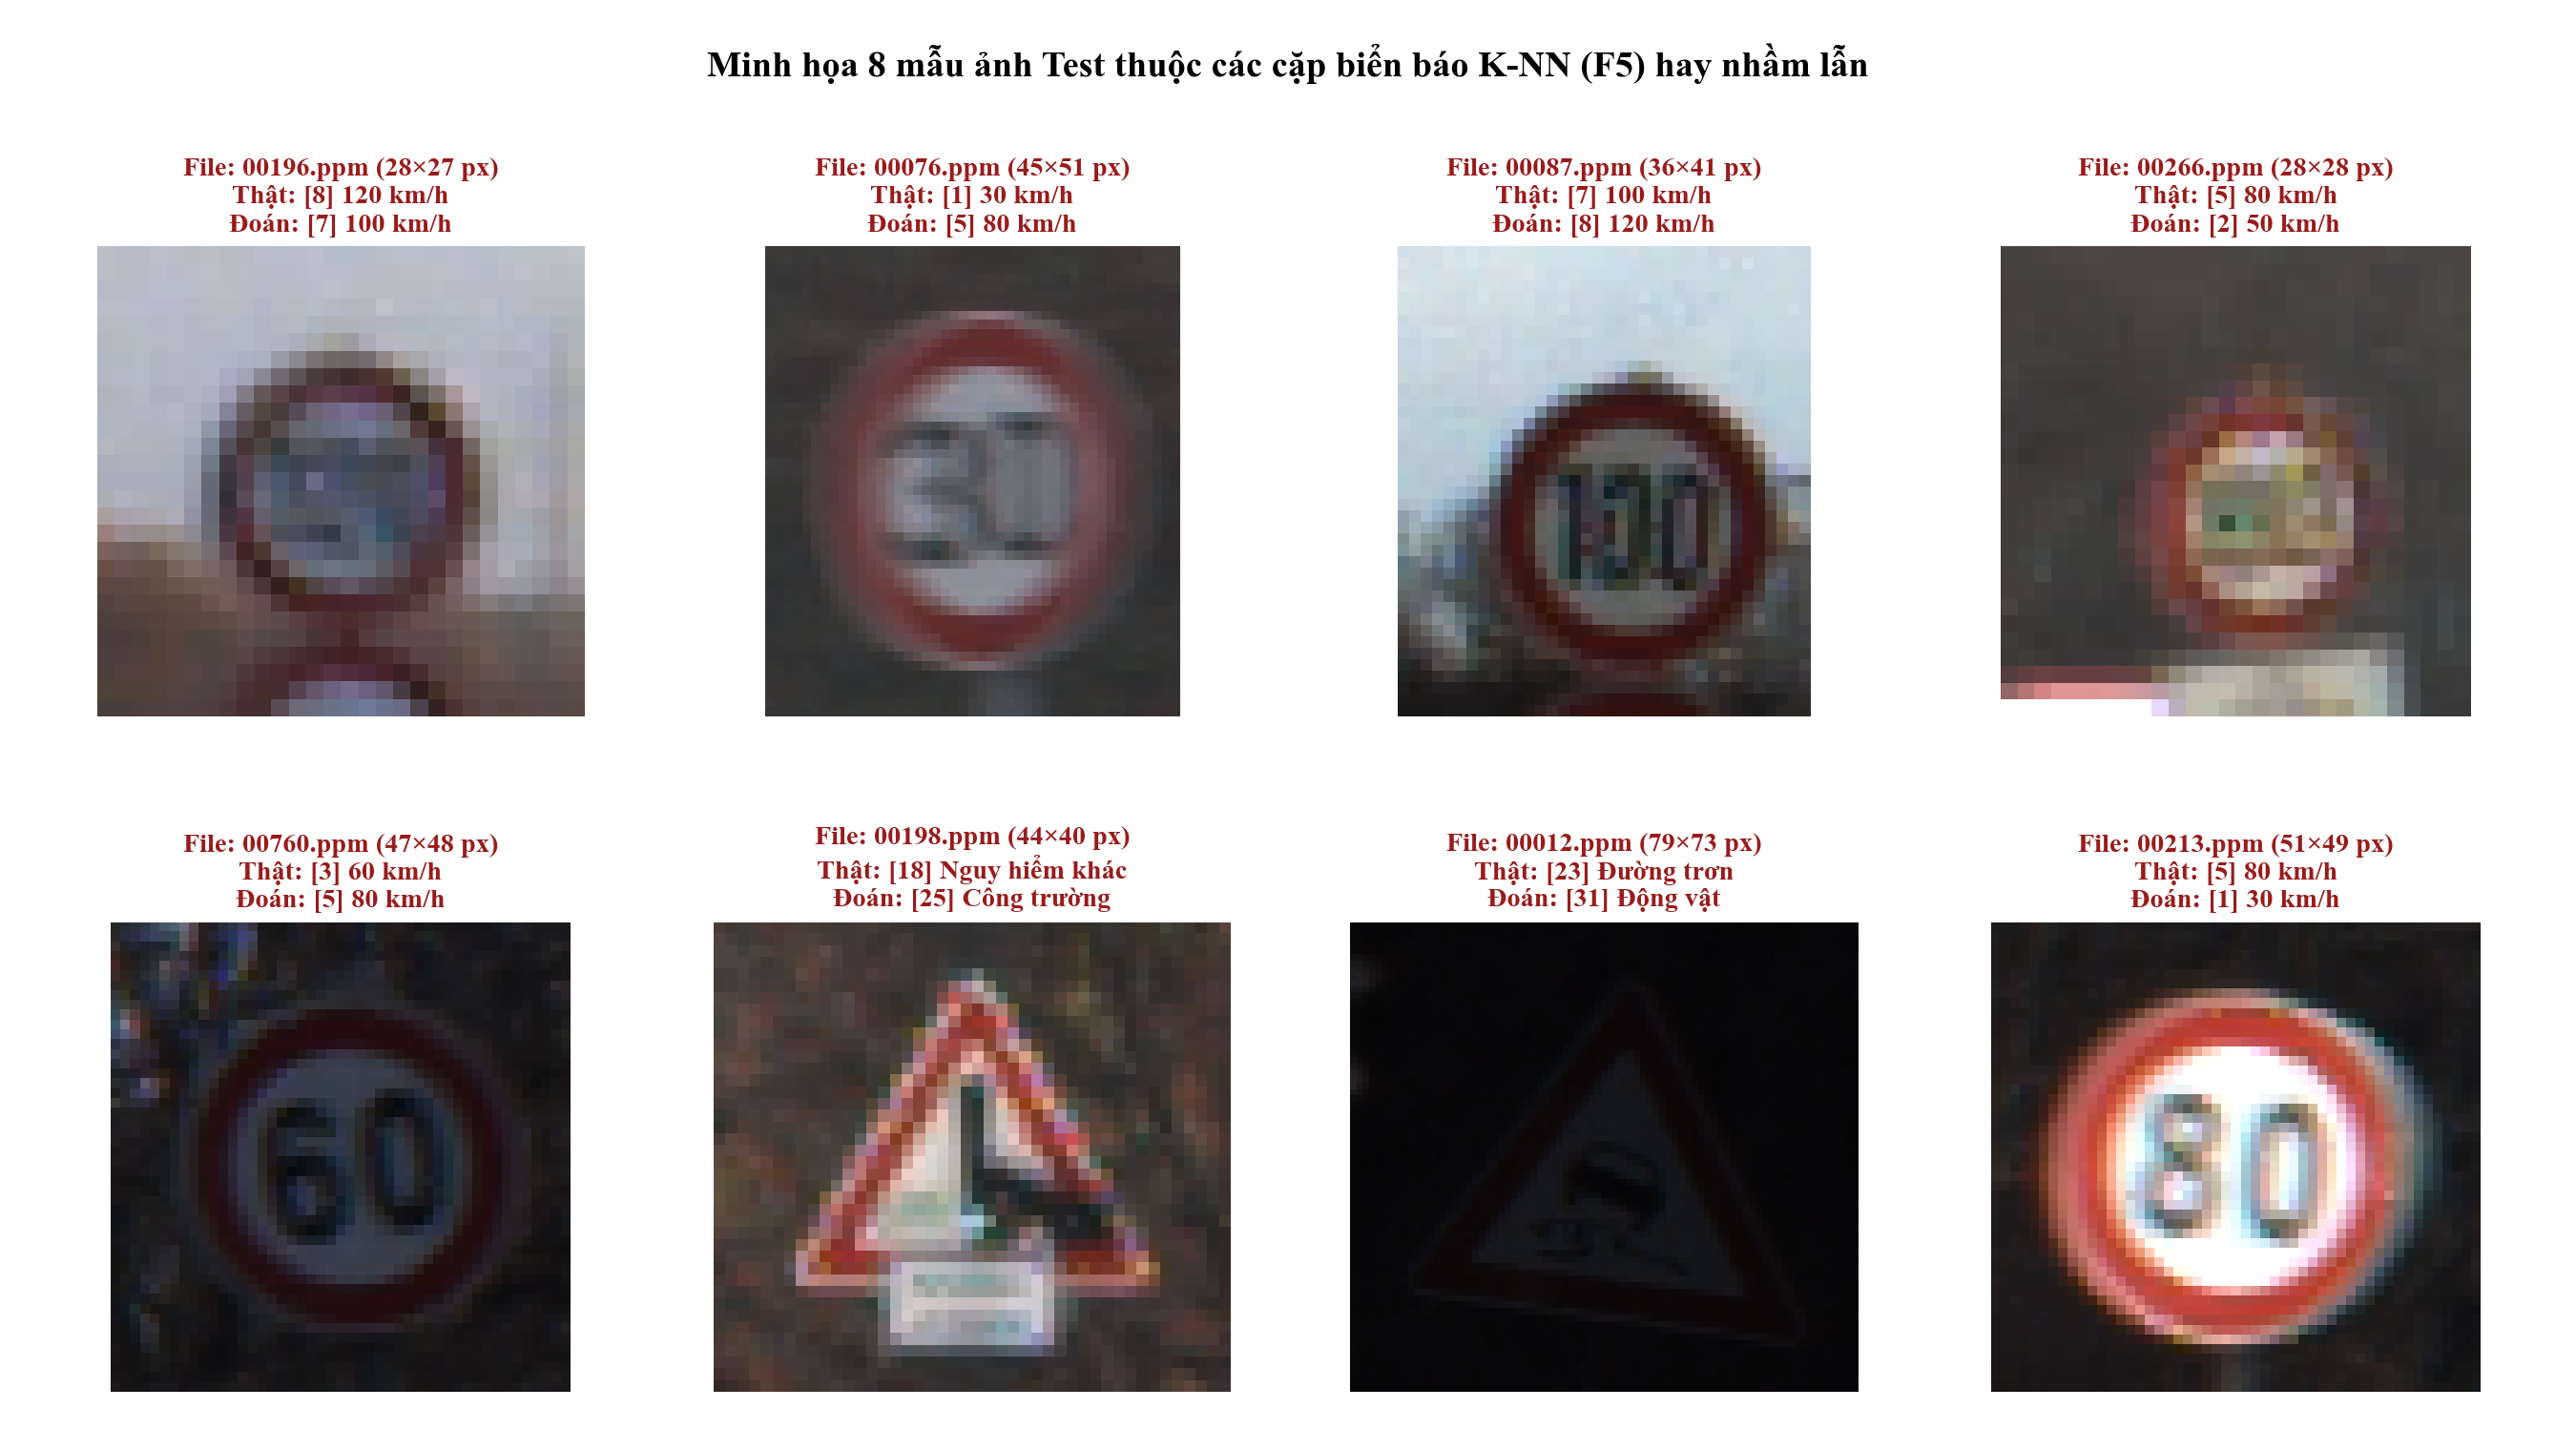
\includegraphics[width=0.56\textwidth]{figures/fig10_error_analysis_samples.png}
\caption{Minh họa 8 mẫu ảnh Test thuộc các cặp lớp hay bị K-NN (F5) dự đoán nhầm.}
\label{fig:err_gallery}
\end{figure*}

Thay vì dừng ở suy đoán trực quan, Hình~\ref{fig:err_diag} kiểm chứng định lượng trên toàn bộ 12.630 ảnh Test:
\begin{enumerate}
  \item Ảnh hưởng của độ phân giải thấp (Hình~\ref{fig:err_diag}a): Nhóm ảnh có chiều rộng nhỏ hơn 32 px (2.105 ảnh) có tỷ lệ lỗi cao tới 16,58\%, cao gấp hơn 2,2 lần nhóm ảnh 46--64 px (7,36\%) và $>$ 64 px (7,69\%), khẳng định định lượng nguyên nhân suy giảm độ nét HOG ở các chữ số tốc độ kích thước nhỏ.
  \item Ảnh hưởng hai đầu của điều kiện sáng (Hình~\ref{fig:err_diag}b): Tỷ lệ lỗi tạo hình chữ U rõ rệt giữa vùng ánh sáng tối cực đoan ($<$ 50: 12,90\%, n=3.821) và vùng chói sáng ($>$ 150: 13,31\%, n=1.142) so với vùng ánh sáng tiêu chuẩn 101--150 (7,20\%).
  \item Hiệu quả ngưỡng từ chối Coverage--Accuracy (Hình~\ref{fig:err_diag}c): Trong bài toán an toàn ADAS (nhằm tránh nhầm 30 km/h lên 50/80 km/h), việc đặt ngưỡng điểm tin cậy $\tau = 0{,}70$ giúp K-NN đạt 97,79\% độ chính xác trên 81,1\% số ảnh (tại $\tau = 0{,}85$ đạt 99,30\% trên 70,3\% ảnh); trong khi MLP tại $\tau = 0{,}95$ duy trì độ phủ 90,3\% với độ chính xác 97,41\%.
\end{enumerate}

Hệ thống hiện còn bốn hạn chế kỹ thuật: (i) phụ thuộc tọa độ ROI cắt sẵn ở tập dữ liệu chuẩn; (ii) lưới HOG/Màu cố định $4\times 4$ nhạy với góc xoay nghiêng lớn; (iii) K-NN phải lưu toàn bộ 31.349 vector huấn luyện; và (iv) tỷ lệ phát hiện lớp thiểu số ở Random Forest bị giảm khi không cân bằng trọng số lớp.

% ==================== SECTION VI ====================
\onecolumn\twocolumn
\section{TỔNG KẾT VÀ HƯỚNG PHÁT TRIỂN}
Nghiên cứu đã xây dựng quy trình nhận dạng biển báo giao thông GTSRB 43 lớp không rò rỉ dữ liệu theo track thông qua StratifiedGroupKFold(5) và chỉ mở khóa đánh giá tập Test một lần ở bước so sánh cuối kèm Bootstrap 95\% CI và kiểm định McNemar. Kết quả thực nghiệm chứng minh đặc trưng hình dạng HOG + CLAHE giữ vai trò quyết định nâng K-NN từ 50,59\% lên 90,45\% (F3-PCA) và 89,79\% (F5), Gaussian Naive Bayes đạt 88,20\% nhanh gấp 5 lần, còn mạng MLP đạt 92,77\% (Macro-F1 89,96\%) trên chỉ 128 chiều PCA. Bốn hướng phát triển tiếp theo gồm: (1) tích hợp bộ phát hiện khung ROI tự động trước phân loại; (2) áp dụng biểu quyết liên khung hình theo chuỗi thời gian (track-level temporal smoothing); (3) thử nghiệm trọng số lớp cân bằng cho Random Forest; và (4) kết hợp kiến trúc mạng nơ-ron tích chập gọn nhẹ để thu hẹp khoảng cách với ngưỡng nhận dạng của con người (98,84\%).

% ==================== REFERENCES ====================
\IEEEtriggeratref{6}
\begin{thebibliography}{16}

\bibitem{stallkamp2011german}
J.~Stallkamp, M.~Schlipsing, J.~Salmen, and C.~Igel, ``The German Traffic Sign Recognition Benchmark: A multi-class classification competition,'' in \textit{Proc. Int. Joint Conf. Neural Netw. (IJCNN)}, 2011, pp.~1453--1460.

\bibitem{stallkamp2012man}
J.~Stallkamp, M.~Schlipsing, J.~Salmen, and C.~Igel, ``Man vs. computer: Benchmarking machine learning algorithms for traffic sign recognition,'' \textit{Neural Netw.}, vol.~32, pp.~323--332, 2012.

\bibitem{kaufman2012leakage}
S.~Kaufman, S.~Rosset, C.~Perlich, and O.~Stitelman, ``Leakage in data mining: Formulation, detection, and avoidance,'' \textit{ACM Trans. Knowl. Discov. Data}, vol.~6, no.~4, pp.~1--21, 2012.

\bibitem{pedregosa2011scikit}
F.~Pedregosa \textit{et al.}, ``Scikit-learn: Machine learning in Python,'' \textit{J. Mach. Learn. Res.}, vol.~12, pp.~2825--2830, 2011.

\bibitem{powers2020evaluation}
D.~M.~W. Powers, ``Evaluation: From precision, recall and F-measure to ROC, informedness, markedness and correlation,'' \textit{arXiv:2010.16061}, 2020.

\bibitem{bradski2000opencv}
G.~Bradski, ``The OpenCV Library,'' \textit{Dr. Dobb's J. Softw. Tools}, vol.~25, no.~11, pp.~120--125, 2000.

\bibitem{zuiderveld1994contrast}
K.~Zuiderveld, ``Contrast limited adaptive histogram equalization,'' in \textit{Graphics Gems IV}, Academic Press, 1994, pp.~474--485.

\bibitem{dalal2005histograms}
N.~Dalal and B.~Triggs, ``Histograms of oriented gradients for human detection,'' in \textit{Proc. IEEE CVPR}, vol.~1, 2005, pp.~886--893.

\bibitem{walt2014scikit}
S.~Van der Walt \textit{et al.}, ``scikit-image: image processing in Python,'' \textit{PeerJ}, vol.~2, p.~e453, 2014.

\bibitem{jolliffe2016principal}
I.~T. Jolliffe and J.~Cadima, ``Principal component analysis: A review and recent developments,'' \textit{Phil. Trans. R. Soc. A}, vol.~374, no.~2065, p.~20150202, 2016.

\bibitem{cover1967nearest}
T.~Cover and P.~Hart, ``Nearest neighbor pattern classification,'' \textit{IEEE Trans. Inf. Theory}, vol.~13, no.~1, pp.~21--27, 1967.

\bibitem{han2011data}
J.~Han, M.~Kamber, and J.~Pei, \textit{Data Mining: Concepts and Techniques}, 3rd ed. Morgan Kaufmann, 2011.

\bibitem{breiman1984classification}
L.~Breiman, J.~Friedman, C.~J. Stone, and R.~A. Olshen, \textit{Classification and Regression Trees}. CRC Press, 1984.

\bibitem{mitchell1997machine}
T.~M. Mitchell, \textit{Machine Learning}. McGraw-Hill, 1997.

\bibitem{breiman2001random}
L.~Breiman, ``Random forests,'' \textit{Mach. Learn.}, vol.~45, no.~1, pp.~5--32, 2001.

\bibitem{grinberg2018flask}
M.~Grinberg, \textit{Flask Web Development: Developing Web Applications with Python}, 2nd~ed. O'Reilly Media, 2018.

\end{thebibliography}

\end{document}